% Spicetracks: Projektbericht Hands-on HCI
% Gruppe 4, Universität St. Gallen, Herbstsemester 2026
% Kompilieren aus diesem Ordner: latexmk -pdf bericht.tex  (oder zweimal pdflatex bericht.tex)
% Die Abbildungen liegen in ../abbildungen/.

\documentclass[11pt,a4paper]{article}

\usepackage[T1]{fontenc}
\usepackage[utf8]{inputenc}
\usepackage[ngerman]{babel}
\usepackage{lmodern}
\usepackage{microtype}
\usepackage[a4paper,margin=2.5cm]{geometry}
\usepackage{graphicx}
\usepackage{float}
\usepackage[font=small,labelfont=bf]{caption}
\usepackage{booktabs}
\usepackage{tabularx}
\usepackage{xltabular}
\usepackage{array}
\usepackage{enumitem}
\usepackage[table]{xcolor}
\usepackage{textcomp}
\usepackage{xurl}
\usepackage{tikz}
\usetikzlibrary{positioning,arrows.meta}
\usepackage[hidelinks]{hyperref}

\graphicspath{{../abbildungen/}}
\setlength{\parindent}{0pt}
\setlength{\parskip}{0.6em}
\renewcommand{\arraystretch}{1.25}
\newcolumntype{L}{>{\raggedright\arraybackslash}X}

% Stellen, die vor der Abgabe noch gefüllt werden müssen
\newcommand{\offen}[1]{%
  \par\noindent\colorbox{yellow!25}{\parbox{\dimexpr\linewidth-2\fboxsep}{\small\textbf{Offen:} #1}}\par}

\title{\textbf{Spicetracks: Projektbericht Hands-on HCI}\\[0.5em]
  \large Hands-on HCI: Entwicklung von Software- und Hardware-Prototypen\\
  Universität St.\,Gallen, Herbstsemester 2026\\
  Dozierende: Katerina Koleva, Leon Reicherts und Gianluca Ielpo}
\author{Gruppe 4: Thierry Suhner, Lukas Kapferer, Phil Solenthaler und Karla Ruggaber}
\date{November 2026}

\begin{document}

\maketitle

\textbf{Relevante Links:}
\begin{itemize}
  \item Github repository: \url{https://github.com/KarlaRuggaber/hands-on-HCI}
  \item Produkt-Video: \url{https://youtu.be/8oCQXXJ95Fs}
  \item Behind the scenes: \url{https://youtu.be/qCuY9ZzWwgk}

\end{itemize}

\tableofcontents
\newpage

% ---------------------------------------------------------------
\section{Kurzfassung}

Spicetracks ist eine interaktive, vollautomatische Kräuterbox für die Küche, in der vier Pflanzen wachsen und die gleichzeitig Musik macht. Die Idee dahinter ist einfach: Frische Kräuter brauchen regelmässig Pflege und gehen trotzdem oft ein, weil man sie vergisst. Musik läuft beim Kochen dagegen sowieso nebenher. Spicetracks verbindet beide Welten. Die Pflanzen sind die Bedienung für die Musik, und wer Musik hören will, hat dadurch automatisch mit seinen Kräutern zu tun. 

In der Box wachsen Basilikum, Oregano, Currykraut und Zimtblätter. Jede Pflanze hat ihre eigene Spotify-Playlist und ihr eigenes Farbschema. Tippt man eine Pflanze an, startet ihre Playlist. Nochmals kurz antippen pausiert die Musik.

Über den Töpfen spannt sich ein Ast aus dem 3D-Drucker, in dem ein LED-Streifen verläuft. Über das Licht zeigt die Box, was gerade passiert. Startet die Musik, breitet sich das Licht von der angetippten Pflanze über den ganzen Ast aus und leuchtet in ihrer Farbe. Auch ihr Topf leuchtet, die anderen bleiben dunkel. So sieht man sofort, welche Pflanze gerade „spielt“. Ist es still, wandert über den Verlauf des Tages eine Sonne über den Ast, und die Lichter an den Töpfen zeigen, wie es den Pflanzen geht: Grün heisst gut versorgt, oranges Pulsieren heisst Durst.

Ums Giessen kümmert sich die Box selbst. Sie misst die Feuchte in jedem Topf und giesst aus dem eingebauten Tank, jede Pflanze nach ihrem eigenen Bedarf, aber nie nachts, weil man die Pumpe sonst hören würde. Dafür reicht eine einzige Pumpe, denn ein Schrittmotor schwenkt den Schlauch über die Pflanze, die Wasser braucht.

Wer genauer wissen will, wie es den Pflanzen geht, schaut aufs Display in der Frontplatte. Dort laufen der Player mit Cover und Lautstärke und für jede Pflanze eine Karte mit Bodenfeuchte, Zustand und dem Zeitpunkt des letzten Giessens. Über das Display kann man auch von Hand giessen, oder die Box in den Nachtmodus schicken.

Technisch besteht der Prototyp aus zwei Geräten. Ein ESP32-S3 liest die Sensoren aus und steuert Pumpe, Motor und LEDs. Ein Raspberry Pi 4 ist für die Logik, Spotify und die Oberfläche zuständig. Beides sitzt in einem Gehäuse aus lasergeschnittenen Holzplatten, die ohne Leim zusammengesteckt sind.

Zu einem der drei vorgeschlagenen Kursthemen kann man Spicetracks nicht eindeutig zuordnen, stattdessen kombiniert es mehrere unterschiedliche Konzepte. Ein Alltagsgegenstand bekommt digitale Funktionen, Sensoren arbeiten mit einem Online-Dienst zusammen, und mit etwas Physischem bedient man etwas Digitales.

\subsection{Team}

Wir sind Gruppe 4: Thierry Suhner, Lukas Kapferer, Phil Solenthaler und Karla Ruggaber. Jede und jeder von uns hatte einen Schwerpunkt (siehe Tabelle), so streng war das in der Praxis aber nicht. Die Aufgaben wechselten oft, wir haben uns gegenseitig geholfen und immer wieder Arbeiten voneinander übernommen.

\begin{table}[H]
\centering
\begin{tabularx}{\linewidth}{lL}
\toprule
\textbf{Person} & \textbf{Schwerpunkt} \\
\midrule
Phil Solenthaler & Wasserverteilung, LED-Strips löten \\
Lukas Kapferer & Elektronik, Verkabelung, Schaltkreis \\
Karla Ruggaber & Elektronik, Verkabelung, Schaltkreis \\
Thierry Suhner & Software, Pläne für 3D-Druck und Lasercutter \\
\bottomrule
\end{tabularx}
\end{table}

Code, Steckplan sowie die Laser- und 3D-Druckdateien liegen im GitHub-Repository \url{https://github.com/KarlaRuggaber/hands-on-HCI}. Wie die Box in Aktion aussieht, zeigt unser Produktvideo (\url{https://youtu.be/8oCQXXJ95Fs}), und wie sie entstanden ist, ein Video hinter den Kulissen (\url{https://youtu.be/qCuY9ZzWwgk}).


% ---------------------------------------------------------------
\section{Motivation}

Am Anfang stand eher ein Wunsch als ein konkretes Problem. Als Team wollten wir etwas bauen, das Spass macht und im Alltag ein lustiger Begleiter ist. Ausserdem sollte möglichst viel unterschiedliche Hardware und Technik darin stecken. Besonders gereizt hat uns die Touch-Funktion. Wir wollten verstehen, wie man so etwas selbst umsetzt, und haben die Herausforderung gerne angenommen. Im Kurs gab es Sensoren, Aktoren, einen Lasercutter und 3D-Drucker, und wir wollten möglichst viel davon ausprobieren. Deshalb kommen in Spicetracks Touch- und Feuchtesensoren, eine Pumpe mit Schrittmotor, adressierbare LEDs, ein Display und Spotify in einem Gerät zusammen.

Die Box soll ein Erlebnis sein, mehr als nur ein Nutzen-Objekt. Sie bringt zwei Dinge zusammen, die es in vielen Wohnungen sowieso gibt: Kräuter, die regelmässig Pflege brauchen, und Musik, die nebenher läuft. Wer die Kräuter berührt, um Musik zu hören, hat mit ihnen also öfter zu tun als nur beim Giessen.

\subsection{Für wen die Box gedacht ist}

Spicetracks ist für alle gedacht, die gerne kochen und Musik hören. Wer frische Kräuter in der Küche hat, kennt das: Sie brauchen regelmässig Wasser, und spätestens in den Ferien vertrocknen sie, weil niemand giesst. Genau da hilft die Box. Sie misst die Feuchte in jedem Topf und giesst selbst aus dem eingebauten Tank, jede Pflanze so viel, wie sie wirklich braucht. Solange Wasser im Tank ist, sind die Kräuter auch versorgt, wenn niemand zu Hause ist.

Dazu kommt, dass viele beim Kochen nebenbei Musik hören. Mit Spicetracks tippt man dafür einfach eine Pflanze an, und die passende Playlist läuft. Das Handy muss man dafür nicht in die Hand nehmen.

Ob jemand die Box allein nutzt oder sie mit anderen teilt, etwa in einer WG oder Familie, spielt für das Konzept keine Rolle.

\subsection{Warum man die Pflanzen berührt}

Beim Kochen hat man selten saubere, freie Hände. Sie sind nass, voller Mehl oder Öl, und das Handy liegt irgendwo ausser Reichweite. Um die Musik zu wechseln, müsste man es entsperren, eine App öffnen und durch Playlists scrollen, mit Fingern, die man gerade nicht auf einen Bildschirm legen möchte. Die Kräuter stehen dagegen ohnehin griffbereit auf der Arbeitsfläche, und beim Kochen greift man sowieso immer wieder zu ihnen. Ein kurzer Tipp auf ein Blatt reicht, egal wie die Hände gerade aussehen. Man muss nichts entsperren, nicht genau zielen und kaum hinschauen.

Wir sehen darin aber mehr als einen bequemeren Schalter. Wer die Pflanzen für die Musik berührt, hat sie öfter in der Hand und merkt dabei nebenbei, wie es ihnen geht: ob die Erde trocken ist, ob Blätter gelb werden oder ob es Zeit zum Ernten ist. Basilikum und Oregano duften, wenn man ihre Blätter streift, die Bedienung riecht also nach Küche. Und weil jede Pflanze ihre eigene Playlist hat, bekommt sie so etwas wie einen eigenen Charakter. Man wählt nicht „Playlist~3“, sondern entscheidet sich für einen Currykraut-Abend. Genau diese Verbindung zwischen Pflanze und Musik war uns wichtiger als die schnellstmögliche Bedienung.

\subsection{Ideenfindung}

Bis die Idee stand, dauerte es eine Weile. Es gab zu viele Ideen und gleichzeitig zu wenige, die sich in einem einwöchigen Blockkurs wirklich umsetzen liessen. Vieles klang spannend, war in der Zeit aber kaum machbar. Außerdem wollten wir kein Projekt starten, welches bereits am Markt existiert oder wir nicht wirklich selbst verwenden würden.

Gesammelt haben wir die Ideen am Whiteboard (Abbildung~\ref{fig:whiteboard}). Auf der Liste standen unter anderem ein Social Buddy, ein Bewässerungssystem, ein Jogging-Coach mit Brust- oder Handgelenkband, ein Präsentations-Coach mit Aufzeichnung und Feedback, ein Productivity Hub und eine Waage, die Kalorien zählt. Rechts daneben steht, was ein Projekt mitbringen sollte: Sensoren und Aktoren, eine Mischung aus Hard- und Software, einen Anwendungsfall und ein richtiges Produkt.

\begin{figure}[H]
\centering
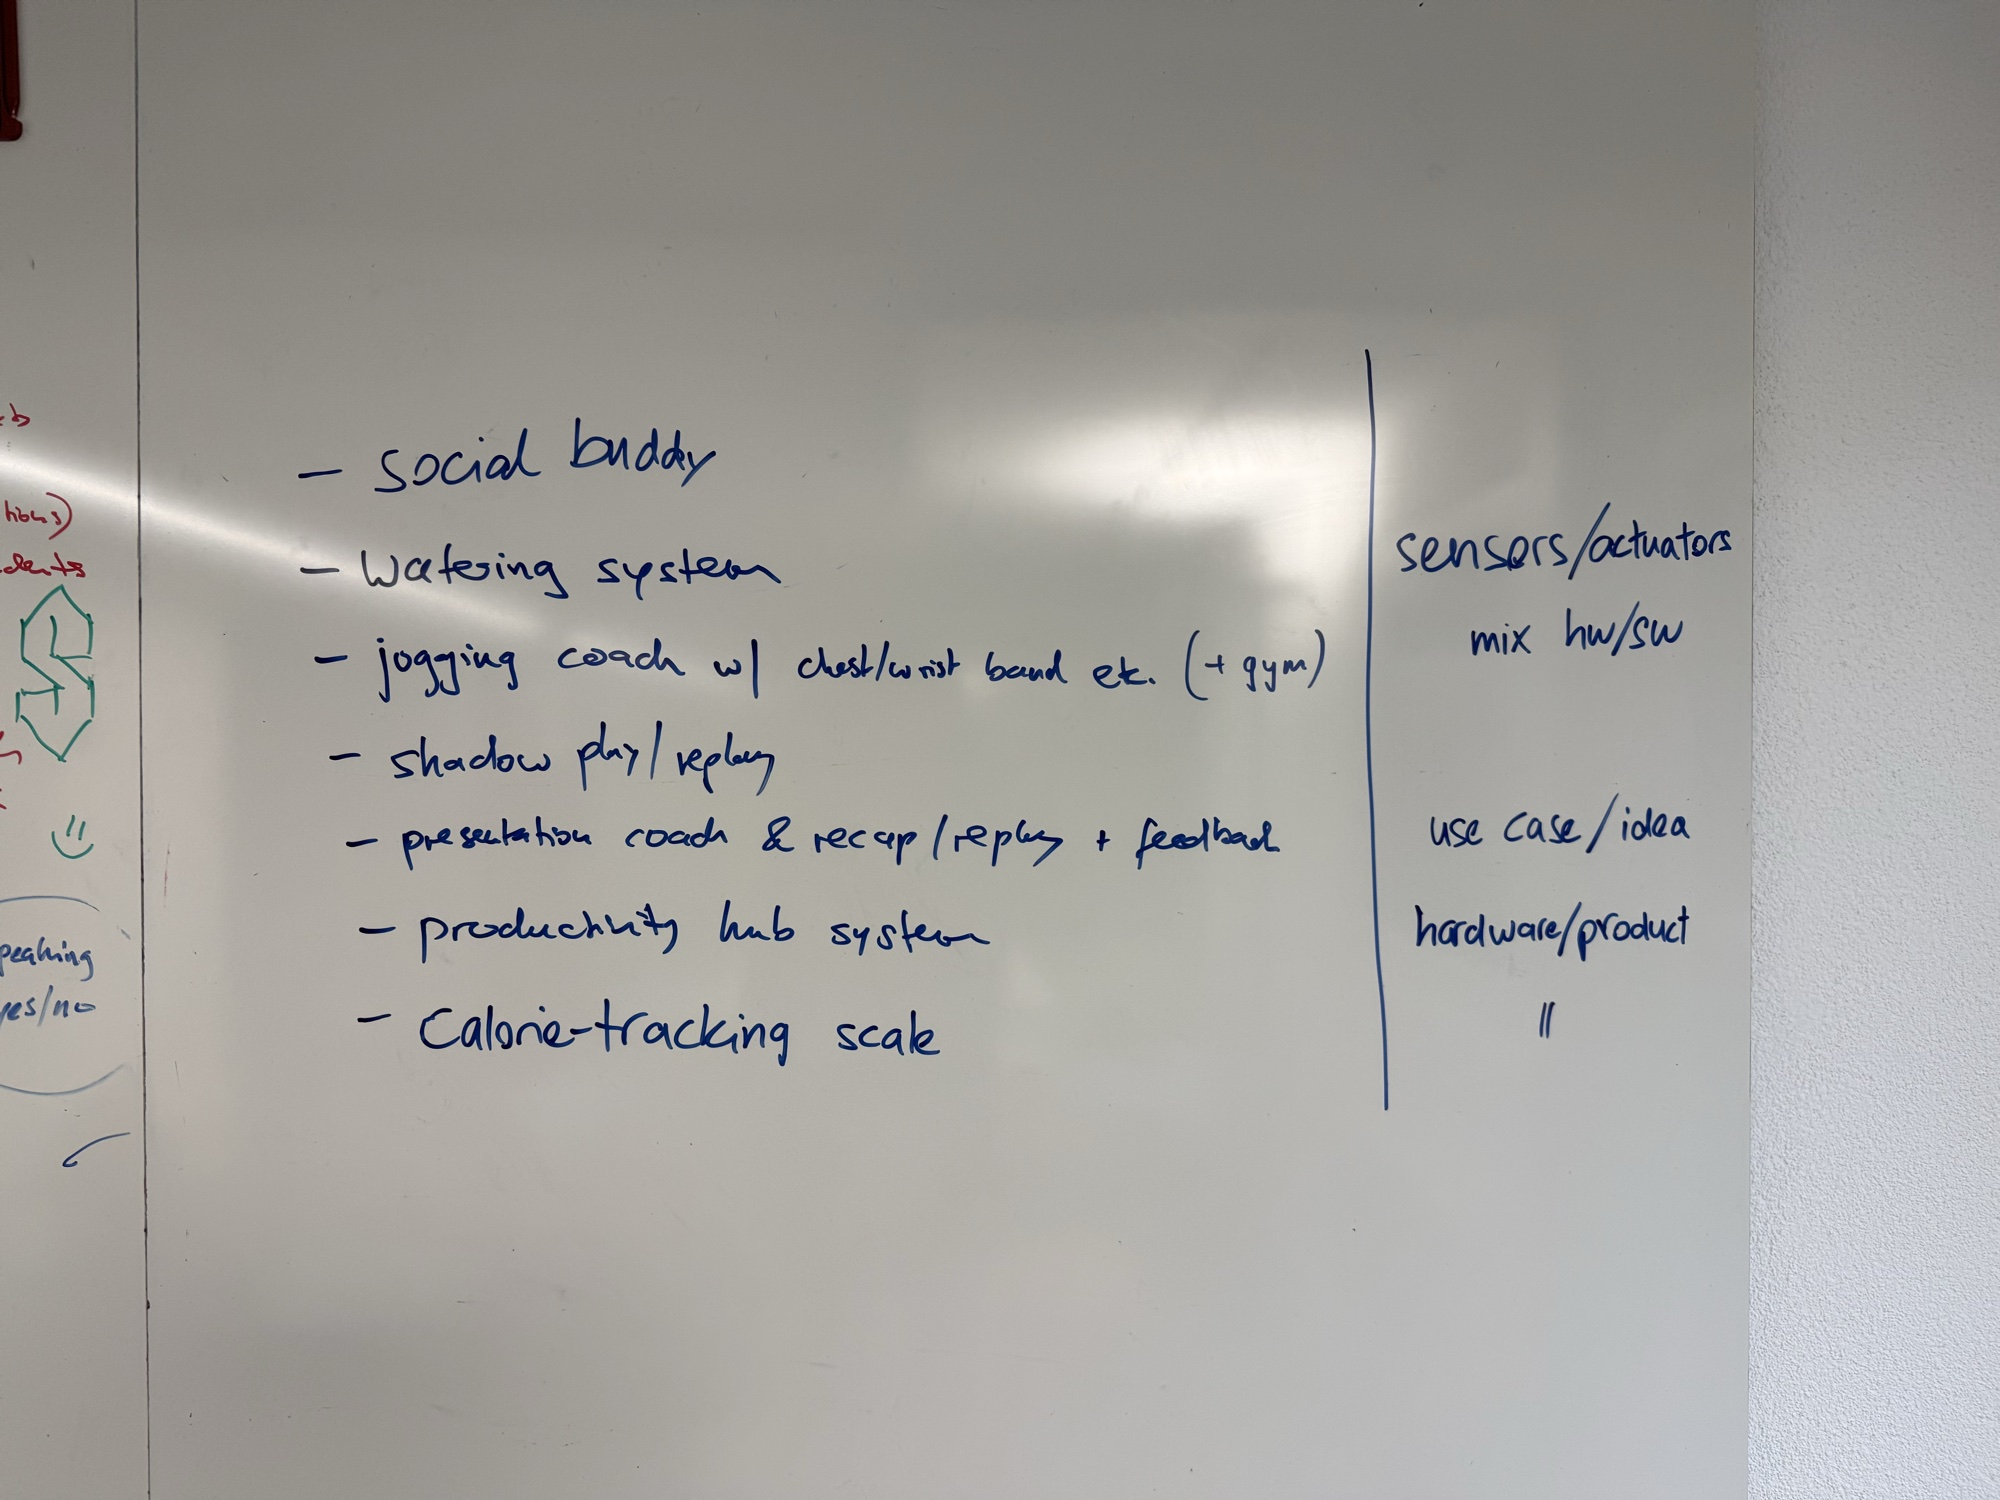
\includegraphics[width=0.75\linewidth]{whiteboard.jpg}
\caption{Ideensammlung am Whiteboard. Rechts stehen die Punkte, die ein Projekt mitbringen sollte.}
\label{fig:whiteboard}
\end{figure}

Um die Liste einzugrenzen, holten wir uns über mehrere Runden Feedback von Leon Reicherts. Mit jeder Runde wurde die Auswahl kleiner, bis ein Konzept übrig blieb, das Spass versprach, sich in der Zeit auch bauen liess und dennoch ausreichend anspruchsvoll war.

Ernsthaft überlegt haben wir uns ausser Spicetracks nur noch den Productivity Hub. Das wäre eine Box gewesen, die beim Arbeiten neben einem auf dem Tisch steht und mit Timer, Uhrzeit und Ähnlichem hilft, produktiv zu bleiben. Entschieden haben wir uns für Spicetracks, weil es die kreativere der beiden Ideen war. Es verbindet etwas, für das wir uns alle begeistern, mit einer Lösung, in der spannende Hard- und Software zusammenkommen.

\subsection{Interaktionsdesign}

Die wichtigste Entscheidung beim Interaktionsdesign war, dass man keine App öffnen muss. Die Pflanzen selbst sind die Tasten. In jedem Topf steckt eine Edelstahlschraube, über die die Box merkt, wenn jemand die Pflanze berührt. Man braucht nur wenige Gesten. Einmal antippen startet die Musik, nochmals kurz antippen pausiert sie. Tippt man eine andere Pflanze an, läuft deren Playlist.

Ohne Knöpfe braucht es eine andere Rückmeldung, und dafür ist das Licht da. Tippt man eine Pflanze an, blitzt ihre Farbe kurz im Trog auf, und wenn gerade keine Musik läuft, auch im Ast darüber. Man weiss also sofort, dass die Berührung angekommen ist. Während Musik läuft, leuchtet nur die Pflanze, die gerade spielt, hell in ihrer Farbe, die anderen Tröge bleiben dunkel. Ohne Musik zeigt das Licht, wie es den Pflanzen geht: ruhiges Grün heisst alles in Ordnung, oranges Pulsieren heisst Durst. Das sieht man auch im Vorbeigehen, ohne aufs Display zu schauen. Wenn eine Pflanze durstig ist, bedeutet dies, dass der Tank vermutlich leer ist.

Dass man dieses Licht versteht, ohne dass es jemand erklärt, hat drei Gründe. Erstens erscheint es genau dort, wo man hingefasst hat. Der Trog der berührten Pflanze blitzt auf, und das Licht im Ast breitet sich von genau dieser Stelle aus. Ursache und Wirkung liegen also direkt beieinander. Zweitens kommt die Rückmeldung sofort, noch bevor die Musik läuft. Spotify braucht nach jedem Befehl einen Moment, und ohne das Licht wüsste man in dieser Pause nicht, ob die Berührung angekommen ist. Viele würden dann nochmals tippen und die gerade startende Musik gleich wieder pausieren. Drittens hat jede Pflanze überall dieselbe Farbe, auf dem Display, am Topf und im Ast. Wer einmal gesehen hat, dass das Basilikum grün und die Zimtblätter rotbraun leuchten, erkennt die Zuordnung überall wieder. Für den Zustand der Pflanzen nutzen wir Signale, die man aus dem Alltag kennt: Ruhiges Grün heisst alles in Ordnung, und ein oranges Pulsieren zieht wie ein Warnlicht die Aufmerksamkeit auf sich, ohne zu stören.

Um die Pflege muss man sich bewusst nicht kümmern. Die Box misst regelmässig die Feuchte und giesst selbst, nachts aber nicht, weil man die Pumpe hört. Für die Grundfunktionen braucht man das Display nicht, dafür reichen die Pflanzen. Wer mehr wissen will, findet dort aber alle Details, und bedienen lässt sich die Box darüber auch.

Auf dem Display in der Front (Abbildung~\ref{fig:prototyp}, rechts) ist links der Player. Dort sieht man das Cover des aktuellen Songs, Titel und Interpret und aus welcher Pflanzen-Playlist er stammt. Darunter folgen der Fortschrittsbalken, Tasten für Zurück, Play/Pause und Weiter und die Lautstärke. Oben steht ein Mond-Knopf für den Nachtmodus mit welchem man jegliche LEDs, die Soundeffekte und das Display deaktivieren kann. Durch einmaliges Berühren des Displays deaktiviert man den Nachtmodus wieder.

Rechts hat jede Pflanze eine eigene Kachel in ihrer Farbe. Darauf stehen die Bodenfeuchte in Prozent, ein Wort für den Zustand (gut, durstig oder sehr nass) und wann zuletzt gemessen und gegossen wurde. Ein Balken zeigt die Feuchte, eine Markierung darauf den Grenzwert, unter dem gegossen wird. Zwei kleine Symbole zeigen, ob die Touch-Erkennung der Pflanze bereit ist oder zum Beispiel noch kalibriert, und ob der Feuchtesensor gerade misst. Mit den zwei Knöpfen unten auf jeder Kachel startet man die Musik dieser Pflanze oder giesst sie von Hand. Fürs Giessen muss man zweimal tippen, beim ersten Mal fragt der Knopf „Sicher?“. So setzt ein versehentlicher Fingertipp keine Pflanze unter Wasser.

Im Nachtmodus wird der Bildschirm schwarz. Der erste Tipp darauf weckt die Box nur und löst keinen Knopf darunter aus. Verliert der Pi die Verbindung zum ESP32, erscheint unten auf dem Bildschirm eine Warnung.

\subsubsection*{Was diese Bedienung kostet}

Pflanzen als Tasten haben auch Nachteile. Einige davon haben wir abgeschwächt, andere bewusst in Kauf genommen.

Der grösste ist, dass man die Bedienung erst entdecken muss. Einem Knopf sieht man an, dass man ihn drücken kann, einer Pflanze nicht. Wer die Box zum ersten Mal sieht, kommt kaum von selbst auf die Idee, ein Basilikumblatt anzutippen, und dass ein zweiter Tipp pausiert, muss man ausprobieren. Im Moment helfen dabei vor allem das Display, auf dem jede Pflanze mit ihrer Farbe und einem Musik-Knopf erscheint, und eine kurze Erklärung beim ersten Benutzen. Ein kleiner Hinweis an der Box selbst wäre eine naheliegende Verbesserung.

Der zweite Nachteil ist, dass man die Musik auch auslösen kann, ohne es zu wollen. Beim Kochen fasst man die Kräuter ja nicht nur für die Musik an, sondern vor allem, um sie zu ernten. Wer ein paar Blätter Basilikum abzupft, startet dabei unter Umständen dessen Playlist oder pausiert sie. Ganz verhindern lässt sich das nicht, denn für den Sensor ist ein Griff zum Ernten dasselbe wie ein Tipp. Wir haben es aber deutlich seltener gemacht. Eine Berührung zählt erst, wenn sie 0,2\,s dauert, die Schwellen sind so hoch, dass eine Hand in der Nähe der Pflanze nichts auslöst, und wer eine Pflanze anfasst, löst nur diese aus und nicht auch die Nachbarn. Passiert es doch, ist der Schaden klein: Ein zweiter Tipp pausiert die Musik wieder. Ausserdem reagiert die Box auf jede Hand, auch auf die von Kindern oder Gästen, die einfach neugierig an den Pflanzen zupfen.

Drittens kann die Bedienung über die Pflanzen nur wenig. Starten, pausieren und zu einer anderen Pflanze wechseln geht. Für die Lautstärke oder einen bestimmten Song braucht man weiterhin das Display. Das ist Absicht, denn jede weitere Geste wäre noch schwerer zu entdecken und noch leichter aus Versehen auszulösen. Die Pflanzen übernehmen deshalb nur das, was man beim Kochen am häufigsten braucht.

Mit Knöpfen wäre die Box eindeutiger zu bedienen, sie wäre dann aber im Grunde ein Lautsprecher mit Kräutern daneben. Gerade dass man die Pflanzen selbst anfasst, macht sie zum Teil des Erlebnisses. Dafür nehmen wir diese Nachteile in Kauf.

% ---------------------------------------------------------------
\section{Der Prototyp}

\begin{figure}[H]
\centering
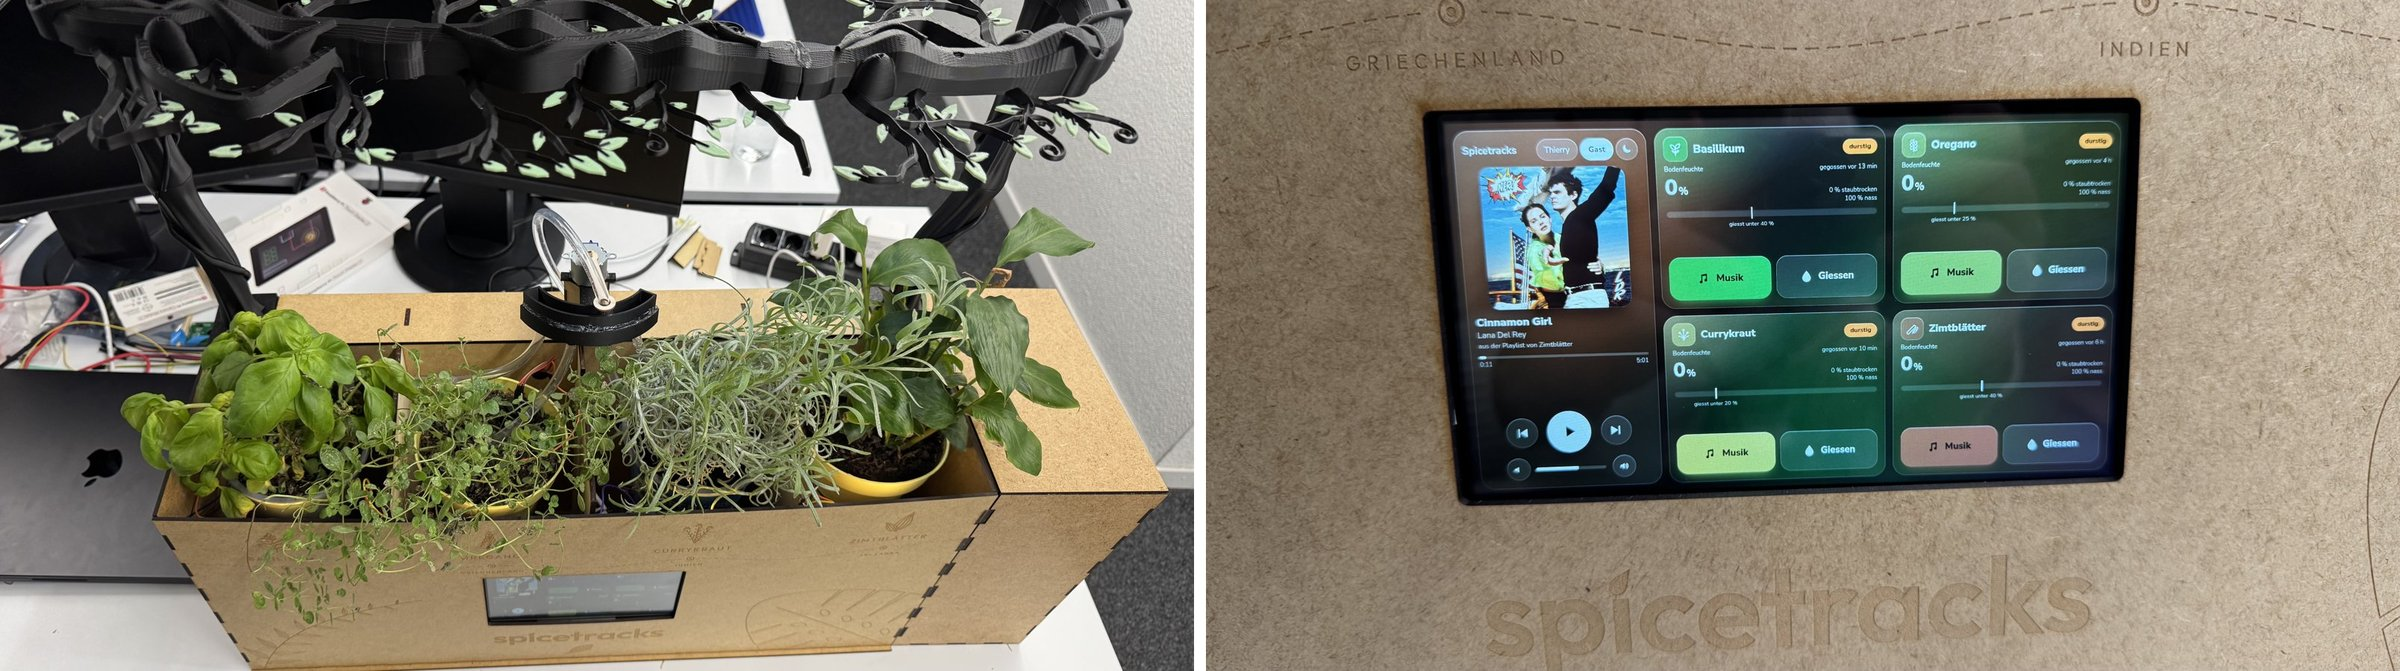
\includegraphics[width=\linewidth]{prototyp.jpg}
\caption{Der fertige Prototyp mit den Kräutern und dem LED-Ast (links) und die Oberfläche auf dem Display in der Front (rechts).}
\label{fig:prototyp}
\end{figure}

Das fertige Produkt reagiert auf folgende Dinge: 
\begin{table}[H]
\centering
\begin{tabularx}{\linewidth}{>{\raggedright\arraybackslash}p{4.6cm}L}
\toprule
\textbf{Aktion} & \textbf{Reaktion} \\
\midrule
Pflanze antippen & Die Playlist dieser Pflanze startet. Ihr Trog leuchtet in ihrer Farbe, im Ast breitet sich das Licht von dieser Pflanze aus. \\
Spielende Pflanze kurz antippen & Pause, danach Ruhelicht \\
Pausierte Pflanze antippen & Musik läuft weiter \\
Andere Pflanze antippen & Wechsel zu deren Playlist \\
Feuchte unter dem Grenzwert & Automatisch giessen, höchstens alle 6\,h pro Pflanze, nicht zwischen 22 und 7 Uhr \\
Mond-Knopf auf dem Display & Nachtmodus: Musik pausiert, LEDs aus, Display schwarz. Ein Tipp auf Display oder Pflanze weckt alles wieder. \\
\bottomrule
\end{tabularx}
\end{table}

\subsection{Licht}

Über das Licht gibt die Box die meisten Rückmeldungen. Es sind insgesamt 40 LEDs, 28 im Ast und je drei innen am Trog jeder Pflanze.

Solange keine Musik läuft, wandert über den Tag eine weiche Sonne von links nach rechts über den Ast. Morgens ist sie rötlich, mittags warmweiss und abends orange, nachts bleibt nur ein schwacher blauer Mond. Die LEDs am Trog zeigen in der Zeit, wie es der jeweiligen Pflanze geht. Grün heisst gut versorgt, oranges Pulsieren heisst Durst, Blau heisst sehr nasse Erde. Schwaches Weiss bedeutet, dass es noch keinen Messwert gibt. Ein Lichtsensor oben am Ast misst ausserdem die Raumhelligkeit, und die Box passt das Ruhelicht daran an.

Startet die Musik, breitet sich das Licht von der Stelle über der angetippten Pflanze nach beiden Seiten aus. Ihr Trog leuchtet hell und pulsiert mit dem Bass, die Tröge der anderen Pflanzen sind aus. Bei Pause zieht sich das Licht wieder in die Pflanze zurück. Auch beim Giessen sieht man etwas: Solange eine Pflanze Wasser bekommt, laufen blaue Tropfen über ihre LEDs.

Sobald der Ton läuft, wird der Ast zum Equalizer. Der Bass liegt in der Mitte, die Höhen aussen, und bei jedem Bass-Schlag blitzt der Ast kurz auf. Je lauter die Musik, desto heller wird die Farbe der spielenden Pflanze, von ihrem dunklen über den kräftigen bis zum hellen Farbton. Wie der Pi dafür die Musik analysiert, steht bei Modul~5.

\subsection{Wann gegossen wird}

Die vier Kräuter brauchen sehr unterschiedlich viel Wasser. Basilikum mag gleichmässig feuchte Erde, Currykraut kommt mit sehr wenig aus und verträgt keine Staunässe. Darum hat jede Pflanze einen eigenen Grenzwert, unter dem gegossen wird, und eine eigene Pumpzeit. Beides lässt sich in der Konfiguration ändern.

\begin{table}[H]
\centering
\begin{tabularx}{\linewidth}{lrrL}
\toprule
\textbf{Pflanze} & \textbf{Giessen unter} & \textbf{Pumpzeit} & \textbf{Begründung} \\
\midrule
Basilikum & 40\,\% & 4,0\,s & mag gleichmässig feuchte Erde \\
Zimtblätter & 40\,\% & 3,5\,s & tropisch, feucht, aber nie nass \\
Oregano & 25\,\% & 3,0\,s & mediterran, darf zwischendurch abtrocknen \\
Currykraut & 20\,\% & 2,5\,s & sehr trockenheitsverträglich, mag keine Staunässe \\
\bottomrule
\end{tabularx}
\end{table}

% ---------------------------------------------------------------
\section{Umsetzung}

Spicetracks besteht aus fünf Modulen: Gehäuse, Wasser, Licht, Touch und Musik. Nach dieser Aufteilung lief auch die Arbeit. Jedes Modul wurde erst einzeln aufgebaut und getestet, oft noch lose auf dem Tisch, und kam danach ins Gehäuse und an die anderen Module. Im Folgenden geht es zuerst um den Ablauf der Woche, dann um den Weg von der Skizze zum Steckplan und um den Aufbau des Ganzen. Danach kommen die Module in der Reihenfolge, in der sie entstanden sind.

\subsection{Ablauf der Woche}

Der Kurs lief als Blockwoche von Montag bis Freitag. In der Tabelle steht, wie sich das Projekt über die fünf Tage und danach entwickelt hat.

\begin{table}[H]
\centering
\begin{tabularx}{\linewidth}{lL}
\toprule
\textbf{Tag} & \textbf{Was passiert ist} \\
\midrule
Montag & Einführung in Prototyping, Sensoren und Aktoren, erste Übungen mit Raspberry Pi und Arduino, erste Ideen für das Gruppenprojekt \\
Dienstag & Ideen eingegrenzt, Pitch von Spicetracks mit Feedback, Start am Prototyp \\
Mittwoch & Hacking Day: Module einzeln aufbauen und testen \\
Donnerstag & Hacking Day und Zwischenstand, bei der Demo macht die Touch-Erkennung noch Probleme \\
Freitag & Störung zwischen Feuchtesensoren und Touch gefunden, Lösung eingebaut, finale Demo \\
Danach & Software überarbeitet (Firmware 2.14): Touch-Erkennung, Bedienung und Licht verbessert \\
\bottomrule
\end{tabularx}
\end{table}

\subsection{Von der Skizze zum Steckplan}

Nach der Ideensammlung am Whiteboard hielten wir Spicetracks zuerst in einer groben Skizze fest. Darauf folgte eine genauere Skizze mit allen Bauteilen, die zeigte, wo sie im Gehäuse in etwa sitzen sollen.

Daraus wurde dann ein genauer Steckplan. Darin steht für jedes Kabel der Pin, das Loch auf dem Breadboard und der Kabeltyp. Dazu kommen Regeln fürs Stecken, zum Beispiel nur ohne Strom zu stecken und die Schienen der beiden Breadboards nie zu verbinden. Nach diesem Plan wurde alles gebaut. Er liegt als interaktive HTML-Datei und als PDF bei, und in der HTML-Version kann man jedes Kabel einzeln hervorheben.

\begin{figure}[H]
\centering
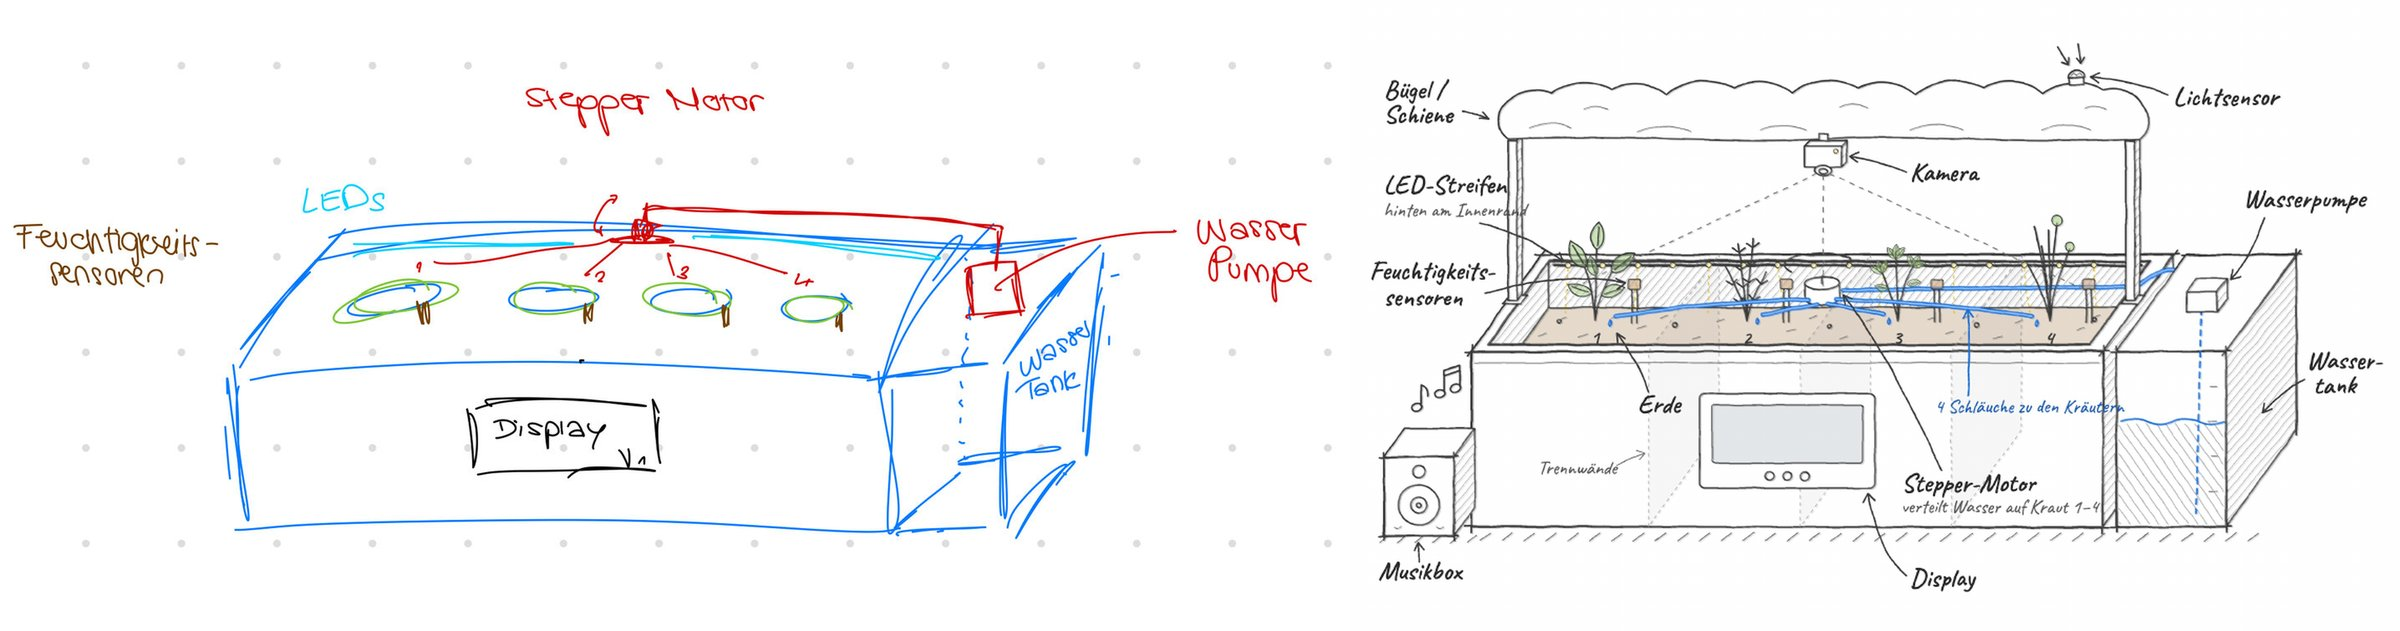
\includegraphics[width=\linewidth]{skizzen.jpg}
\caption{Erste grobe Skizze (links) und genauere Skizze mit allen geplanten Bauteilen (rechts). Manches davon, zum Beispiel die Kamera, wurde später nicht umgesetzt.}
\label{fig:skizzen}
\end{figure}

\begin{figure}[H]
\centering
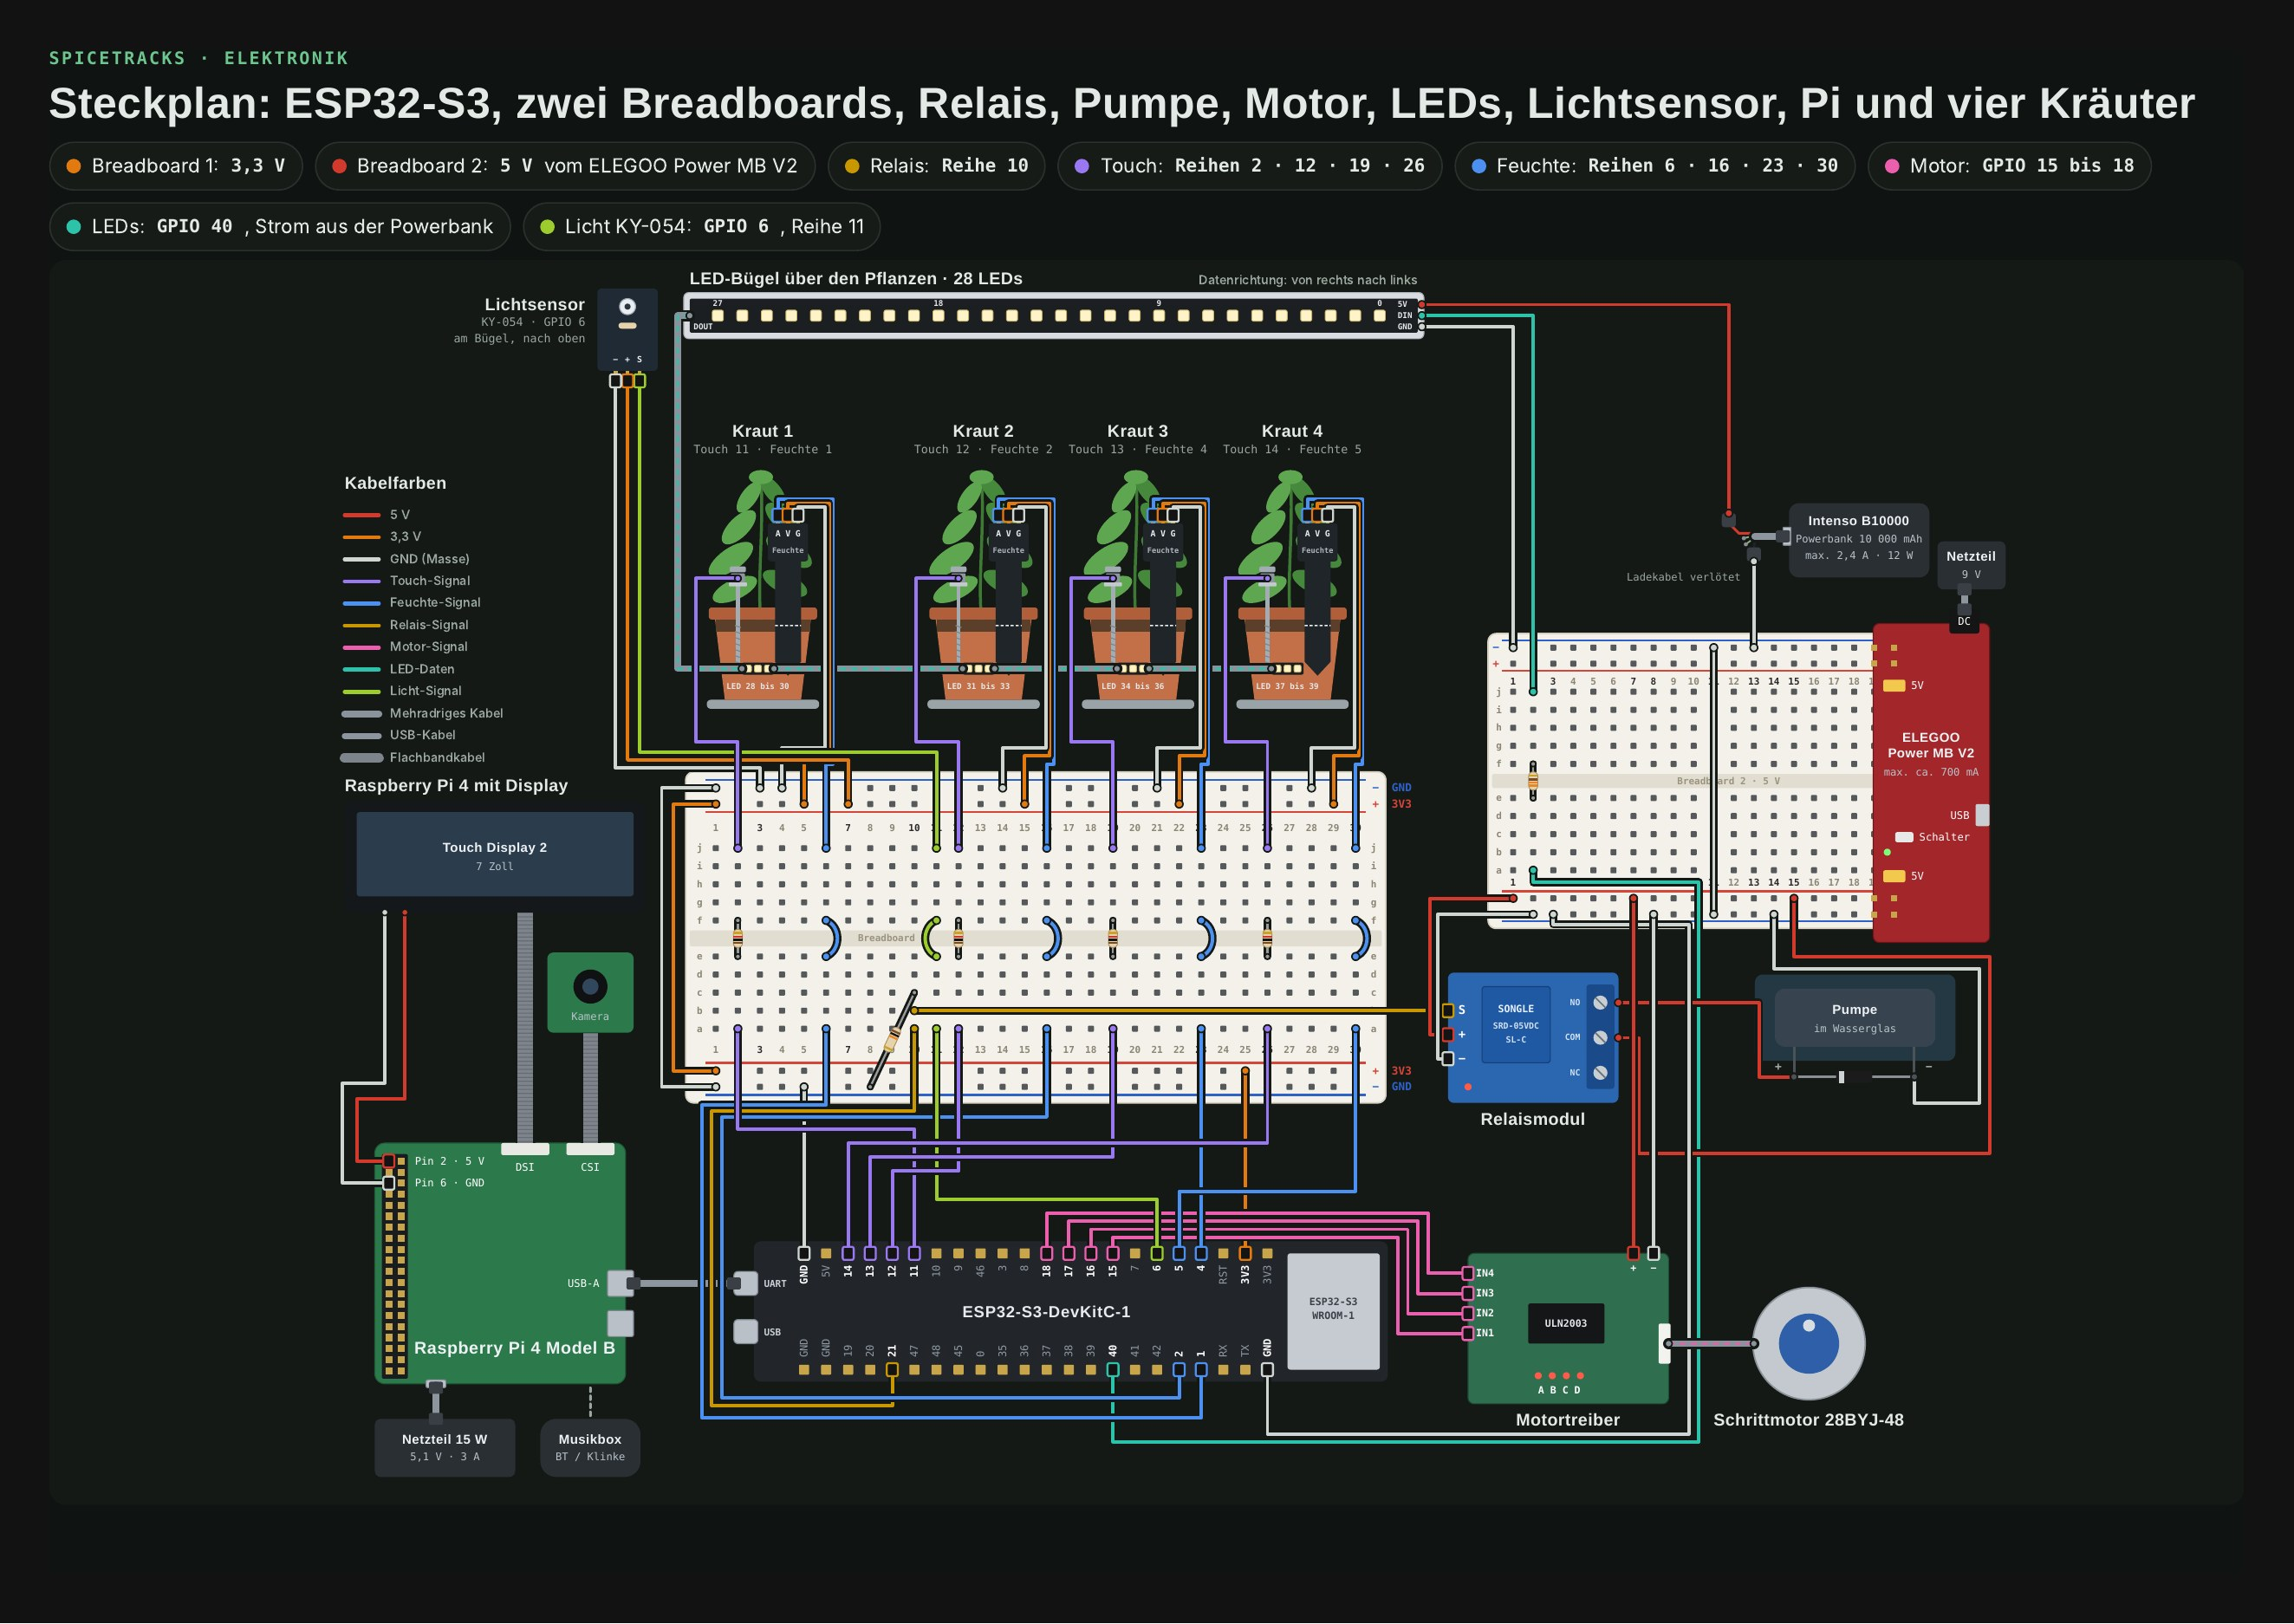
\includegraphics[width=\linewidth]{steckplan.jpg}
\caption{Steckplan mit ESP32-S3, zwei Breadboards, Relais, Pumpe, Motor, LEDs, Lichtsensor, Raspberry Pi und den vier Kräutern. Die vollständige Kabelliste steht in der PDF- und HTML-Version des Steckplans.}
\label{fig:steckplan}
\end{figure}

\subsection{Aufbau im Überblick}

Die Arbeit ist auf zwei Geräte verteilt, und jedes macht das, was es besser kann. Der ESP32-S3 liest die Sensoren aus und steuert Pumpe, Motor und LEDs. Selbst entscheidet er nichts, er macht, was der Pi ihm sagt. Der Raspberry Pi wertet die Messwerte aus, steuert Spotify, berechnet den Equalizer und zeigt die Oberfläche auf dem Display. Verbunden sind die beiden über USB. Sie schicken sich kurze JSON-Nachrichten, eine pro Zeile, mit 115200 Baud.

\begin{figure}[H]
\centering
\resizebox{\linewidth}{!}{%
\begin{tikzpicture}[
    font=\small,
    box/.style={draw=black!45, rounded corners=3pt, text width=3.9cm, minimum height=1.05cm, align=left, inner sep=4pt},
    core/.style={draw=teal!70!black, fill=teal!10, line width=0.9pt, rounded corners=4pt, minimum width=2.9cm, minimum height=8.4cm, align=center},
    arr/.style={-{Stealth[length=2.2mm]}, draw=black!55},
    both/.style={{Stealth[length=2.2mm]}-{Stealth[length=2.2mm]}, draw=black!55}
  ]
  % Mitte: Pi und ESP32
  \node[core] (pi) at (0,0) {\textbf{Raspberry Pi}\\[2pt]\footnotesize Logik\\\footnotesize Spotify-Steuerung\\\footnotesize Equalizer (FFT)\\\footnotesize Weboberfläche};
  \node[core] (esp) at (4.4,0) {\textbf{ESP32-S3}\\[2pt]\footnotesize Sensoren lesen\\\footnotesize Aktoren schalten\\\footnotesize Pumpe stoppt\\\footnotesize nach max.\ 10\,s};
  \draw[both] (pi.east) -- node[above, font=\scriptsize, text=black!65]{USB} node[below, font=\scriptsize, text=black!65]{JSON} (esp.west);

  % Links: was am Pi hängt
  \node[box] (disp) at (-4.4, 2.1) {\textbf{Display}\\\footnotesize Oberfläche im Browser};
  \node[box] (spot) at (-4.4, 0) {\textbf{Spotify}\\\footnotesize Web API, Playback SDK};
  \node[box] (spk)  at (-4.4,-2.1) {\textbf{Lautsprecher}\\\footnotesize per Bluetooth};
  \draw[both] (disp.east) -- (disp.east -| pi.west);
  \draw[both] (spot.east) -- (spot.east -| pi.west);
  \draw[arr]  (spk.east -| pi.west) -- (spk.east);

  % Rechts: was am ESP32 hängt
  \node[box] (touch) at (8.8, 3.5)  {\textbf{Touch}\\\footnotesize Schrauben in den Töpfen};
  \node[box] (moist) at (8.8, 2.1)  {\textbf{Feuchtesensoren}\\\footnotesize nur kurz eingeschaltet};
  \node[box] (light) at (8.8, 0.7)  {\textbf{Lichtsensor}\\\footnotesize Raumhelligkeit};
  \node[box] (pump)  at (8.8,-0.7)  {\textbf{Relais und Pumpe}\\\footnotesize Wasser aus dem Tank};
  \node[box] (motor) at (8.8,-2.1)  {\textbf{Schrittmotor}\\\footnotesize schwenkt den Schlauch};
  \node[box] (leds)  at (8.8,-3.5)  {\textbf{40 RGBW-LEDs}\\\footnotesize Ast und Tröge};
  \foreach \n in {touch,moist,light} \draw[arr] (\n.west) -- (\n.west -| esp.east);
  \foreach \n in {pump,motor,leds} \draw[arr] (\n.west -| esp.east) -- (\n.west);
\end{tikzpicture}}
\caption*{Aufbau: Raspberry Pi, ESP32 und ihre Bauteile}
\end{figure}

Die Pfeile zeigen, in welche Richtung die Daten laufen: Die Sensoren melden an den ESP32, der ESP32 schaltet Pumpe, Motor und LEDs, und entschieden wird auf dem Pi.

Dafür gab es zwei Gründe. Der ESP32 kommt gut mit Aufgaben zurecht, bei denen das Timing stimmen muss, etwa der Touch-Messung und den LEDs. Spotify, die Audioanalyse und die Weboberfläche sind dagegen in Python auf dem Pi viel einfacher. Der zweite Grund ist Sicherheit, falls auf dem Pi etwas schiefgeht. Die Pumpe stoppt immer nach spätestens 10\,s, egal was der Pi schickt. Fällt der Pi ganz aus, zum Beispiel durch einen Absturz oder Neustart, schaltet der ESP32 nach 30\,s ins Ruhelicht und lässt die Pumpe aus.

Die Tabelle fasst alle Bauteile mit ihrer Aufgabe und ihrem Anschluss zusammen.

\begin{table}[H]
\centering
\small
\begin{tabularx}{\linewidth}{>{\raggedright\arraybackslash}p{4.4cm}L>{\raggedright\arraybackslash}p{4.2cm}}
\toprule
\textbf{Bauteil} & \textbf{Aufgabe} & \textbf{Anschluss} \\
\midrule
ESP32-S3-DevKitC-1 & Sensoren lesen, Aktoren steuern & USB zum Pi \\
Raspberry Pi 4 mit Display & Logik, Spotify, Equalizer, Oberfläche & USB zum ESP32 \\
4 Edelstahlschrauben & Touch-Sensoren in den Töpfen & GPIO 11 bis 14 \\
4 Feuchtesensoren & Bodenfeuchte & GPIO 1, 2, 4 und 5, 3,3\,V \\
Lichtsensor KY-054 & Raumhelligkeit & GPIO 6, 3,3\,V \\
Relais und Pumpe & Wasser aus dem Tank fördern & Relais an GPIO 21 \\
Schrittmotor mit ULN2003-Treiber & Arm mit Schlauch zur richtigen Pflanze schwenken & GPIO 15 bis 18 \\
LED-Streifen SK6812 RGBW, 40 LEDs & Ast und Tröge beleuchten & GPIO 40 über 330\,$\Omega$ \\
ELEGOO Power MB V2 & 5\,V für Relais, Motor, Pumpe & Breadboard 2 \\
Powerbank Intenso B10000 & Strom für die LEDs & LED-Streifen \\
Bluetooth-Lautsprecher & Musik & Bluetooth zum Pi \\
\bottomrule
\end{tabularx}
\end{table}

\subsection{Modul 1: Gehäuse}

Zuerst brauchten die Kräuter ein Gehäuse. Es wurde am Lasercutter aus Platten geschnitten. Die Teile greifen mit Fingerzinken ineinander und sind nur gesteckt, nicht geklebt. So lässt sich die Box wieder öffnen, wenn an der Elektronik etwas geändert werden muss.

Damit die Verbindungen auch halten, gab es vorher Probestücke, um zu sehen, wie fest die Fingerzinken bei 3\,mm Material sitzen. Erst dann wurden die richtigen Teile geschnitten. Das fertige Gehäuse hat vier Fächer für die Kräuter, einen Wassertank und ein Fenster für das Display.

Die Schnittdateien sind nach Teilen getrennt: Front, Innenwand, Rückwand, Boden und Deckel, Seitenwände und Tank sowie die Trennwände zwischen den Fächern, die aus 4\,mm dickem Material geschnitten sind. Dazu kommt die Datei für die Probestücke, damit man den Passtest bei einem Nachbau wiederholen kann.

\begin{figure}[H]
\centering
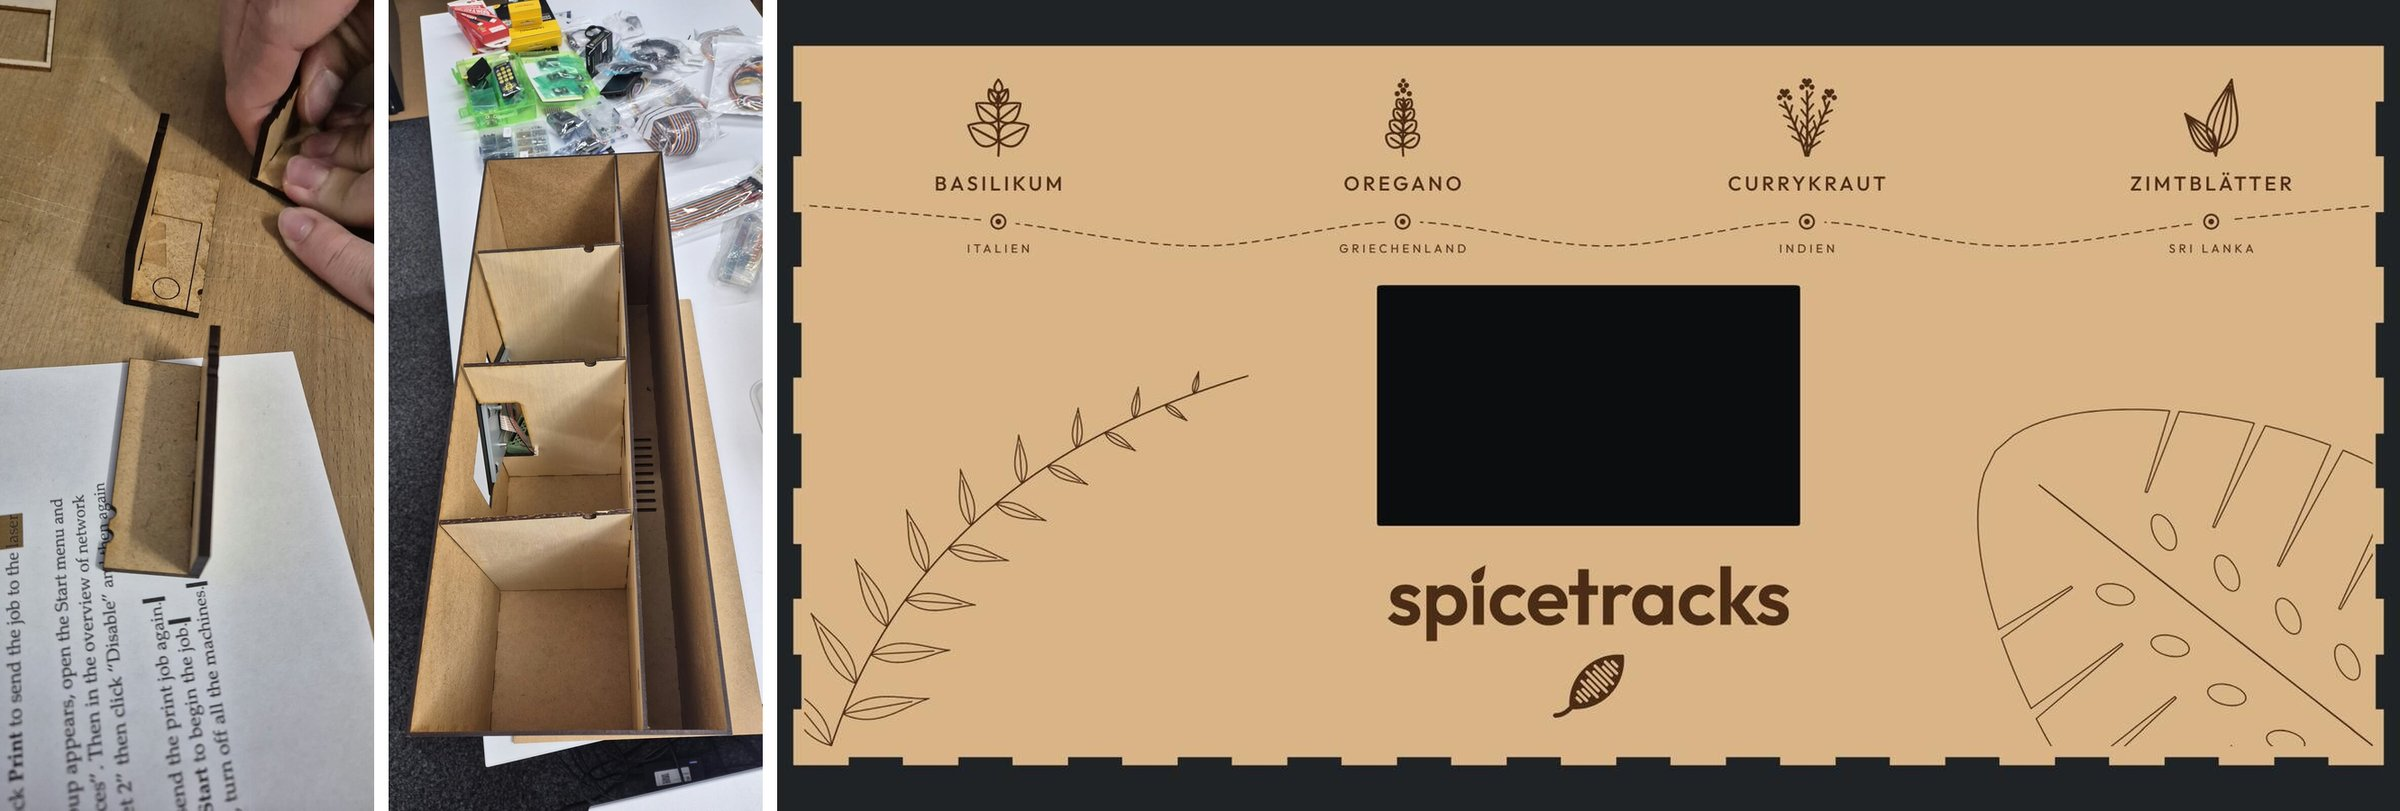
\includegraphics[width=\linewidth]{gehaeuse.jpg}
\caption{Probestück für die Fingerzinken (links), die gesteckten Fächer ohne Leim (Mitte) und der Entwurf der gravierten Front mit dem Fenster für das Display (rechts).}
\label{fig:gehaeuse}
\end{figure}

\subsection{Modul 2: Wasser}

Danach kam das Wasser. Pumpe, Relais und Feuchtesensoren wurden zuerst einzeln getestet, die Pumpe stand dafür noch in einem Wasserglas auf dem Tisch. Als das lief, ging es um die eigentliche Frage: Wie kommt das Wasser von einer einzigen Pumpe zu vier verschiedenen Pflanzen?

Vier Pumpen hätten mehr Platz, mehr Strom und mehr Anschlüsse gebraucht, also blieb es bei einer. Ein Schrittmotor dreht einen kleinen Arm, an dem der Schlauch hängt, und bringt ihn über die Pflanze, die Wasser braucht. Die Positionen der vier Pflanzen sind als Motorschritte gespeichert, bei 515, 345, 170 und 0 Schritten.

Für den Verteiler, über den das Wasser vom Arm in die Töpfe läuft, brauchte es mehrere Drucke, bis die Form stimmte. Das erste, gelbe Teil war ein gerades Stück mit vier Anschlüssen. Gedruckt wurde es vor allem, um zu testen, ob sich die Schläuche sauber anstecken lassen, ohne dass daneben Wasser herausläuft. Am Arm sah man dann aber auch, dass er sich im Halbkreis bewegt und an den beiden Enden am geraden Verteiler vorbeiläuft. Das zweite, schwarze Teil ist deshalb gebogen und folgt genau dem Weg des Arms. Es hat pro Pflanze eine Vertiefung, an der der Arm anhält und das Wasser abgibt.

Beim Giessen arbeiten Pi und ESP32 zusammen. Der Pi entscheidet anhand der Feuchtewerte, wann eine Pflanze Wasser braucht. Dabei giesst er jede Pflanze höchstens alle 6\,h und nie zwischen 22 und 7 Uhr. Dann schickt er dem ESP32 einen Befehl mit der Pflanze und der Pumpzeit. Der ESP32 fährt den Arm an die richtige Stelle, schaltet die Pumpe über das Relais ein und meldet danach, wie lange er gepumpt hat.

Im normalen Betrieb arbeitet die Box mit den echten Messwerten der Feuchtesensoren. Für Vorführungen gibt es zusätzlich einen Demo-Modus. Echte Erde trocknet nur langsam aus, und in einer Präsentation würde man kaum sehen, dass sich etwas tut. Im Demo-Modus startet deshalb jede Pflanze mit einem für sie typischen Feuchtewert, und jedes Giessen erhöht ihn sichtbar um 3 bis 6\,\%. So sieht man auch in wenigen Minuten, wie die Box auf das Giessen reagiert.

\begin{figure}[H]
\centering
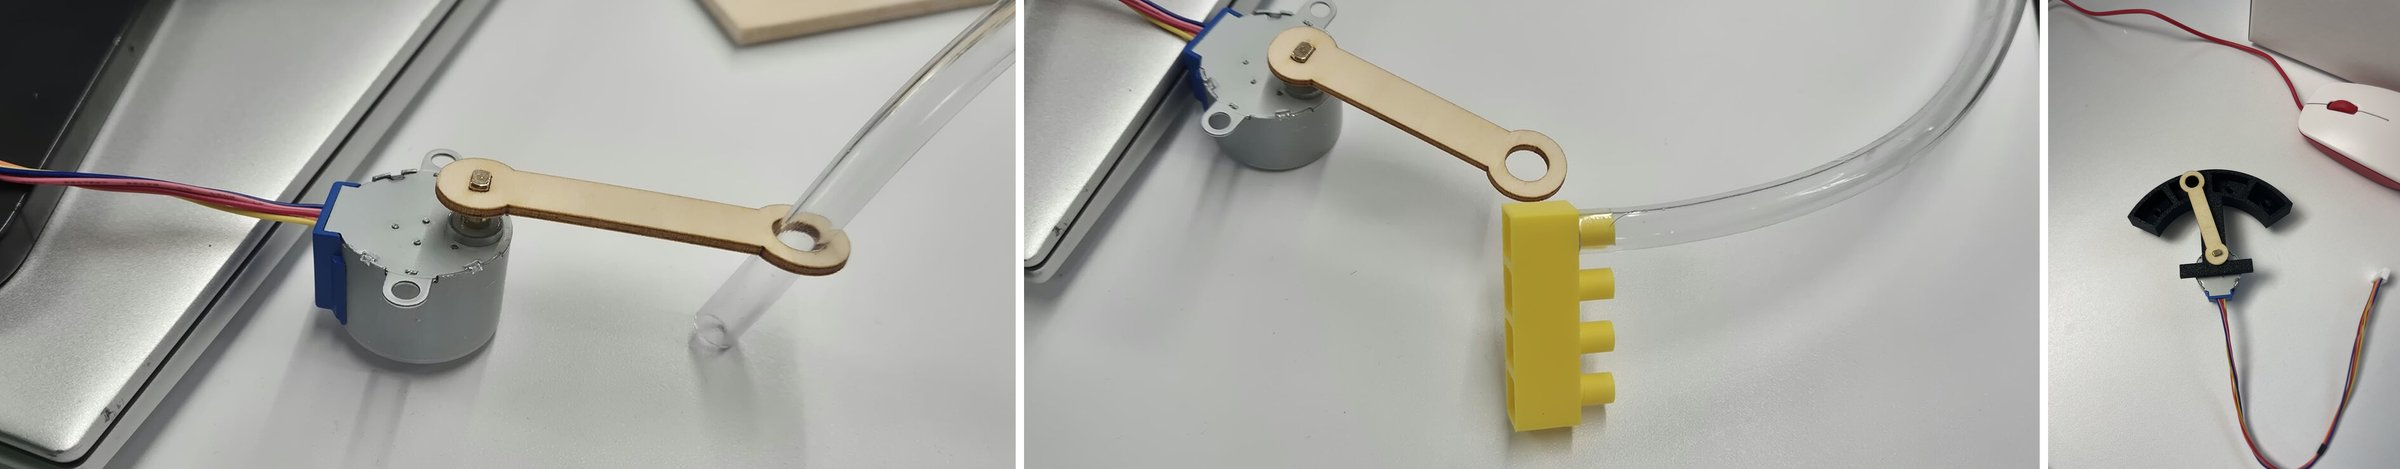
\includegraphics[width=\linewidth]{wasser.jpg}
\caption{Schrittmotor mit Arm (links), der erste, gerade Verteiler in Gelb (Mitte) und der gebogene Verteiler in Schwarz (rechts).}
\label{fig:wasser}
\end{figure}

\subsection{Modul 3: Licht}

Als drittes kam das Licht. Für den Ast über den Kräutern gab es vier Entwürfe mit verschiedenen Formen, gewählt wurde Variante B, die wild gewachsene.

Der Ast war allerdings länger als der Druckraum des 3D-Druckers. Deshalb wurde er in drei Teile zerlegt, die nach dem Druck zusammengesteckt werden. Getragen wird er von zwei Stämmen mit Füssen. Alles zusammen passt auf fünf Druckplatten.

In einer Nut im Ast liegt ein LED-Streifen mit 28 LEDs, der vorher auch erst lose auf dem Tisch getestet wurde. Von dort läuft die gleiche LED-Kette weiter zu den Töpfen, wo je drei LEDs innen am Trog sitzen. Alle 40 LEDs hängen also an einem einzigen Datenpin. Jede LED im Ast kennt ihre Position und damit die Pflanze unter ihr. Deshalb kann sich das Licht von der richtigen Stelle aus ausbreiten, wenn jemand eine Pflanze antippt.

Beim Licht haben wir die meiste Zeit mit Fehlersuche verbracht. Nach dem ersten Löten blieb der Streifen komplett dunkel. Erst nach langem Messen mit dem Multimeter fanden wir die Ursache: Ein Jumperkabel war defekt. Mit einem neuen Kabel leuchteten die LEDs endlich, allerdings nicht in den bunten Farben der Pflanzen, sondern nur in Blau, Rot und Weiss.

Mehrere Stunden lang suchten wir danach den Fehler. Wir prüften Lötstellen und Kabel noch einmal und vermuteten schon, dass der Streifen selbst kaputt ist. Die Lösung lag am Ende ganz woanders. Bestellt war ein RGB-Streifen, geliefert wurde aber ein RGBW-Streifen, der Weiss als vierte Farbe hat. Er kam in einem einfachen Plastiksack ohne Beschriftung, deshalb ist das beim Auspacken niemandem von uns aufgefallen. Ein RGBW-Streifen erwartet pro LED 4 Byte statt 3. Die Firmware schickte aber nur 3, also rutschten die Farbwerte von LED zu LED weiter, und ein Teil davon landete auf dem weissen Chip. Kaputt war also gar nichts. Sobald die Firmware auf RGBW umgestellt war, stimmten die Farben, ohne dass an der Hardware etwas geändert werden musste.

Schwierig war auch die Stromversorgung. Bei voller Helligkeit brauchen 40 LEDs deutlich mehr Strom, als das Netzteil-Modul auf dem Breadboard liefert, denn das schafft nur etwa 700\,mA. Die LEDs hängen deshalb an einer eigenen Powerbank. Sie liefert höchstens 2,4\,A, und die Firmware begrenzt den Strom der LEDs auf 1,5\,A, damit die Powerbank nicht überlastet wird. 

Dazu kam die gemeinsame Masse. Solange die Masse des ESP32 nicht mit der des zweiten Breadboards verbunden war, schalteten Relais, Motor und LEDs mal richtig und mal nicht. Mit der Verbindung lief dann alles stabil.

\begin{figure}[H]
\centering
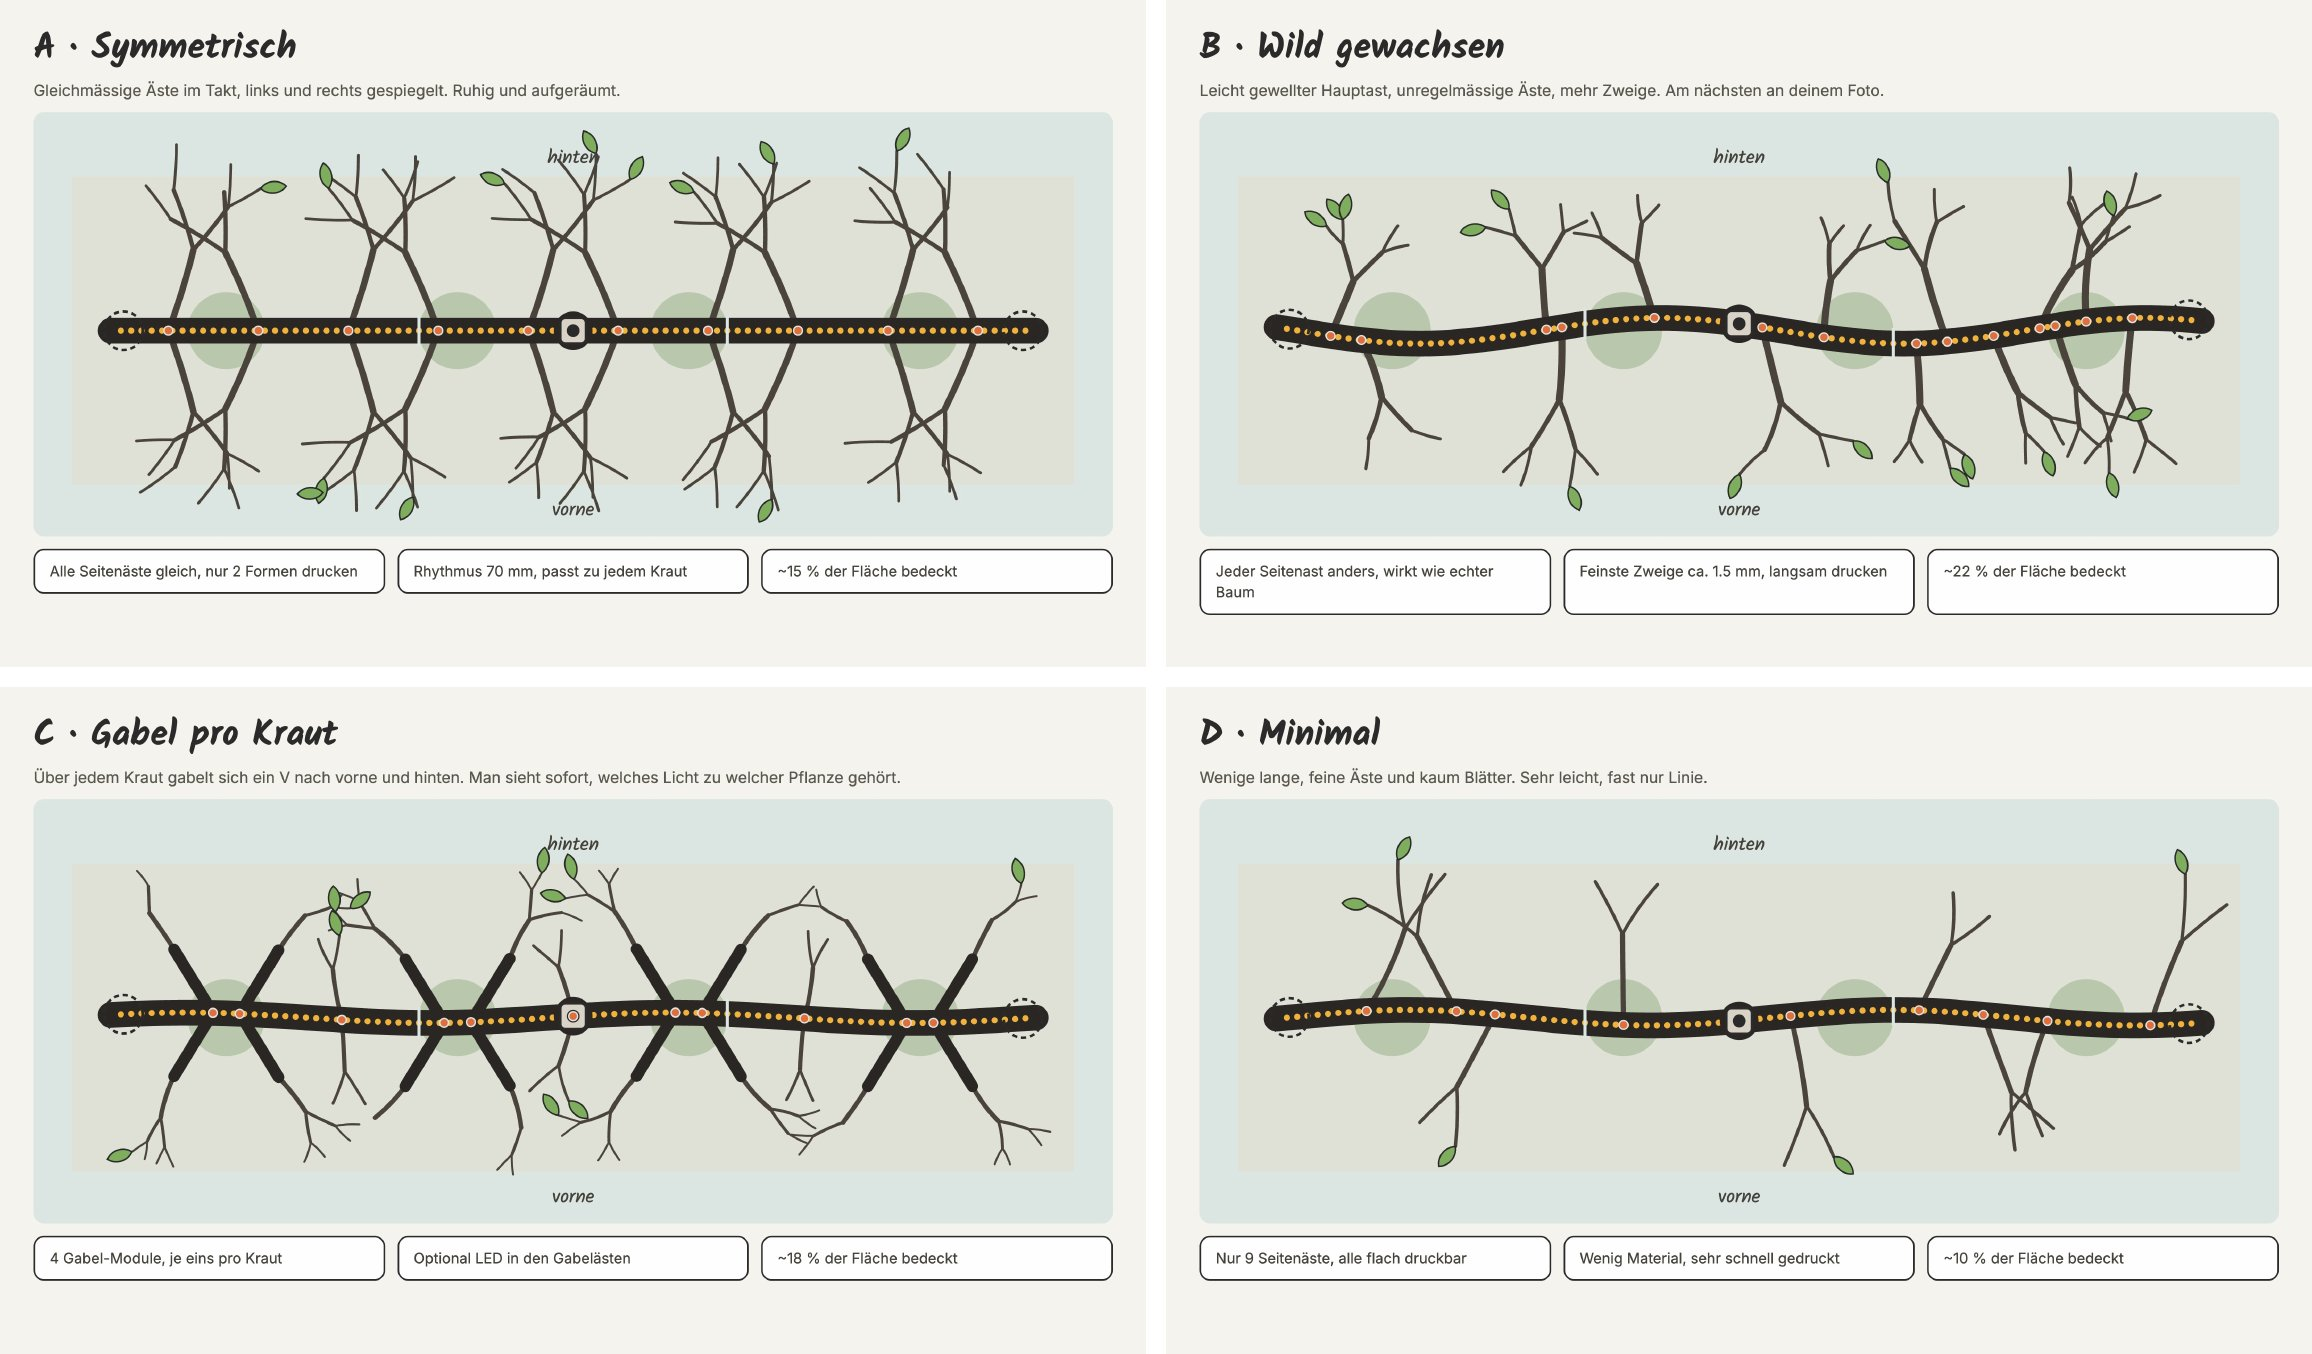
\includegraphics[width=0.85\linewidth]{entwuerfe.jpg}
\caption{Die vier Entwürfe für den Ast. Gewählt wurde Variante B, „Wild gewachsen“ (oben rechts).}
\label{fig:entwuerfe}
\end{figure}

\begin{figure}[H]
\centering
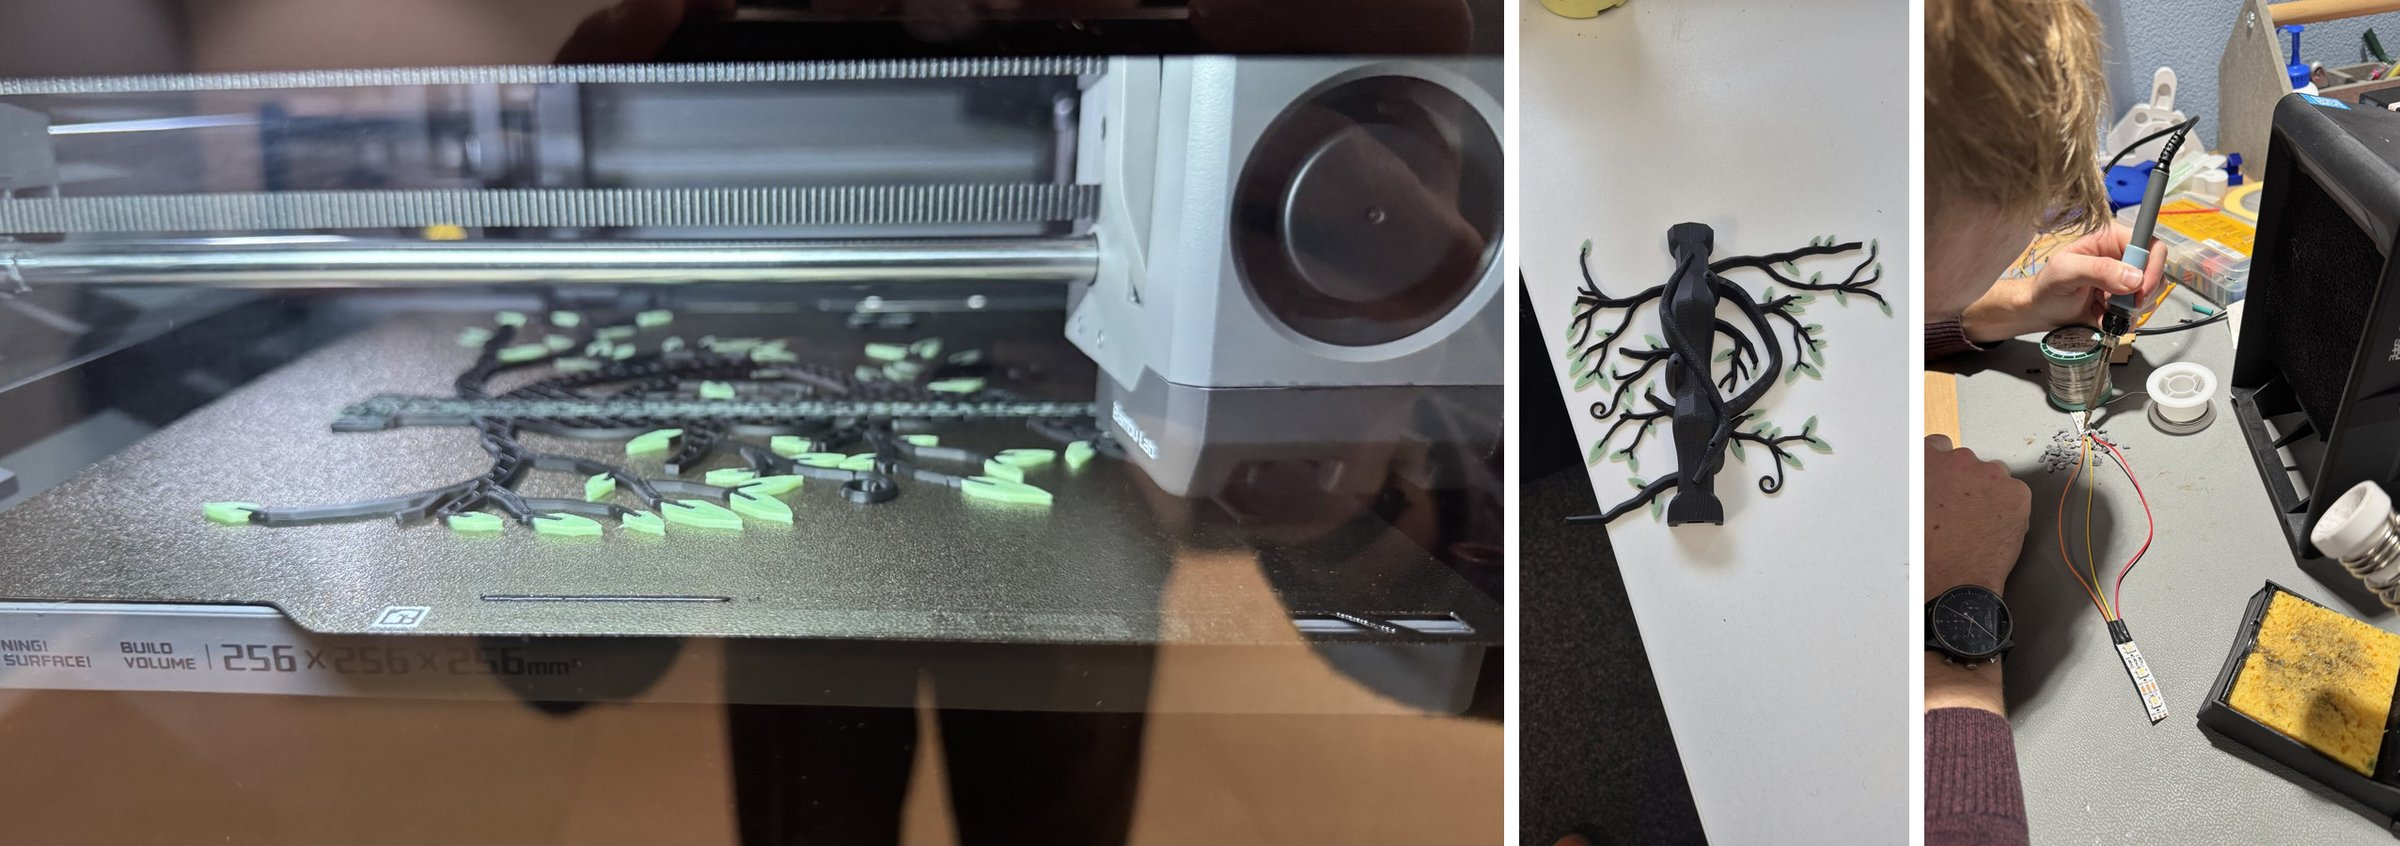
\includegraphics[width=\linewidth]{licht.jpg}
\caption{Druck der Ast-Teile im 3D-Drucker (links), ein gedrucktes Ast-Teil (Mitte) und Löten am LED-Streifen (rechts).}
\label{fig:licht}
\end{figure}

\subsection{Modul 4: Touch}

Mit dem vierten Modul werden die Kräuter zu Tasten. In jedem Topf steckt dafür eine Edelstahlschraube in der Erde, die an einem Touch-Pin des ESP32 hängt. Berührt jemand die Pflanze, ändert der Körper die Kapazität, und der ESP32 misst einen höheren Wert. Die Pflanze und die feuchte Erde leiten die Berührung bis zur Schraube.

Das hat fast zu gut funktioniert. Die erste Version reagierte auch auf das Brummen aus der Steckdose und löste immer wieder von selbst aus, z.B. auch durchs Vorbeigehen. Erst die vierte Version erkennt nur noch echte Berührungen.

Sie misst jeden Kanal 100 Mal im Abstand von 1\,ms und nimmt den Mittelwert über diese 100\,ms. Das sind genau fünf Perioden des 50-Hz-Stromnetzes, so mittelt sich das Brummen heraus. Nach dem Start kalibriert sich die Erkennung 30\,s lang und misst, wie stark der Wert ohne Berührung schwankt. Die Schwelle liegt beim Sechsfachen dieses Rauschens. Als Berührung zählt es erst, wenn der Wert 0,2\,s lang über der Schwelle bleibt, damit kurze Ausreisser nichts auslösen.

Ein zweites Problem tauchte erst auf, als die Module zusammen liefen. Steckte ein Feuchtesensor im selben Topf, reagierte die Pflanze nicht mehr auf Berührungen. Schlimmer noch: Der Touch-Chip hielt dann die Messung für alle vier Pflanzen an. Beim Messen lädt der Chip die Schraube kurz auf und misst, wie lange das dauert. Der Feuchtesensor liegt mit seiner grossen Kupferfläche aber in derselben nassen Erde. Dadurch dauerte das Aufladen so lange, dass der Chip abbrach.

Gelöst haben wir das, indem Feuchte und Touch sich abwechseln. Die Feuchte wird nur noch alle 10 Minuten und 45\,s nach jedem Giessen gemessen, jeweils für etwa 2\,s, und in dieser Zeit pausiert die Touch-Erkennung. Seitdem laufen Feuchtesensoren und Touch problemlos nebeneinander. Hängt ein Kanal trotzdem einmal, meldet die Firmware ihn als „stuck“, und die anderen Pflanzen funktionieren weiter.

Dazu kam ein drittes Problem. Wer eine Pflanze anfasst, lässt oft auch die Nachbartöpfe ausschlagen. Seit Firmware 2.12 gilt deshalb immer nur eine Pflanze als berührt, nämlich die, deren Wert am stärksten über ihrer Schwelle liegt. Eine andere Pflanze übernimmt erst, wenn sie 1,5-mal stärker ausschlägt. Ausserdem lässt sich die Empfindlichkeit in der \path{config.yaml} einstellen. Im Moment sind die Schwellen dreimal so hoch wie nach der Kalibrierung, liegen also beim Achtzehnfachen des Rauschens. So löst auch eine Hand, die nur in die Nähe der Pflanze kommt, nichts mehr aus. Auf dem Pi wird zusätzlich dieselbe Pflanze 2\,s nach einem Musikbefehl ignoriert, damit ein nachfedernder Kontakt die Musik nicht gleich wieder pausiert.

Damit die Touch-Messung den Rest des Systems nicht ausbremst, läuft sie auf dem zweiten Kern des ESP32. So bleiben LEDs und die Verbindung zum Pi flüssig, auch während gemessen wird.

\begin{figure}[H]
\centering
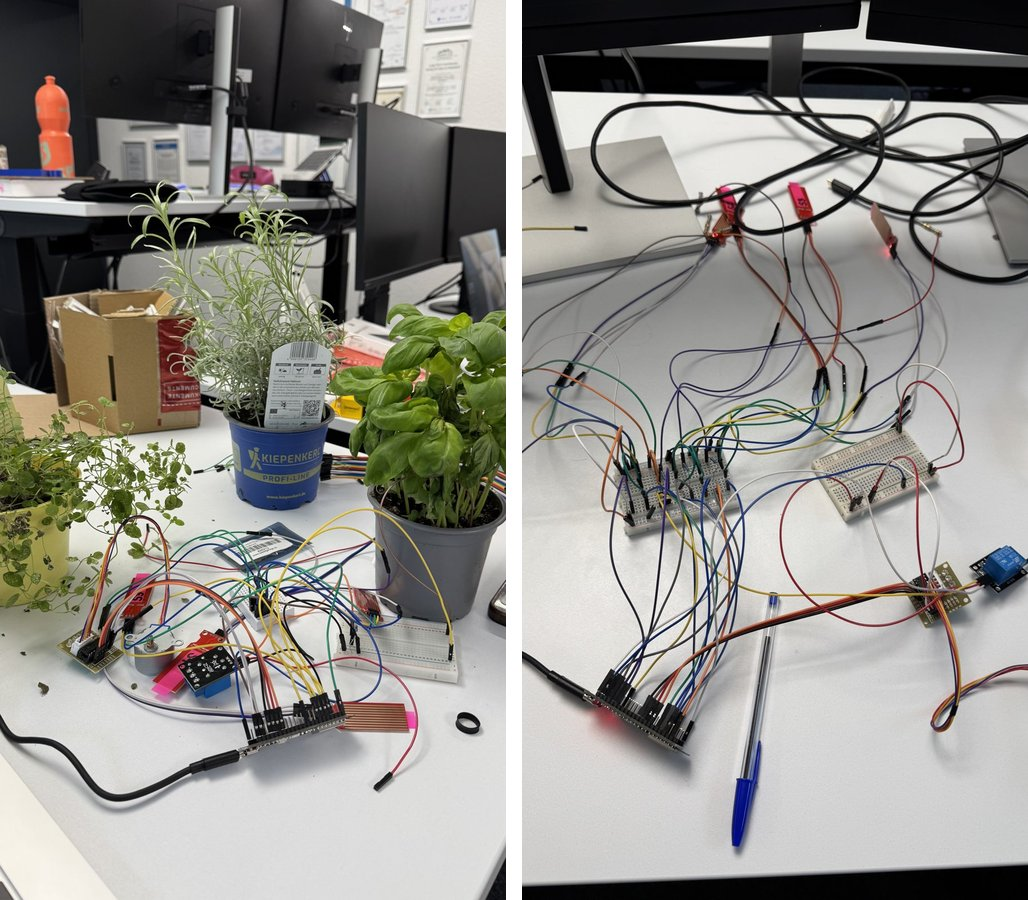
\includegraphics[width=0.6\linewidth]{touch.jpg}
\caption{Erste Tests mit den Kräutern am Breadboard (links) und die Verkabelung während der Tests (rechts).}
\label{fig:touch}
\end{figure}

\subsection{Modul 5: Musik}

Das letzte Modul verbindet die Box mit Spotify, und hier ging es nicht auf direktem Weg. Zuerst sollte librespot die Musik direkt auf dem Pi abspielen, sodass der Pi selbst als Spotify-Lautsprecher auftaucht. Das blockiert Spotify aber, weil es für viele Konten den nötigen Audio-Schlüssel nicht mehr herausgibt.

Funktioniert hat schliesslich eine andere Lösung. Die Musik läuft im Browser auf dem Display, über das offizielle Spotify Web Playback SDK. Damit Chromium geschützte Musik abspielen darf, braucht es zusätzlich das Widevine-Modul. Gesteuert wird alles über die Spotify Web API. Tippt jemand eine Pflanze an, sagt der Pi also nur „spiel Playlist X auf dem Gerät Spicetracks“, und der Browser auf dem Display spielt die Musik ab.

Auch beim Equalizer musste ein anderer Weg her. Geplant war, die Audioanalyse von Spotify zu nutzen, die Takt und Lautstärke eines Songs liefert. Diese Daten gibt Spotify aber seit Ende 2024 an neue Apps nicht mehr heraus. Deshalb hört der Pi selbst mit, was der Lautsprecher gerade spielt, über den PipeWire-Monitor.

Aus diesem Signal berechnet er 30 Mal pro Sekunde per FFT acht Frequenzbänder von 40\,Hz bis 12\,kHz, erkennt die Bass-Schläge und schickt beides an den ESP32. Ein Problem gab es noch mit dem Timing, denn Bluetooth-Lautsprecher hängen 150 bis 250\,ms hinterher. Das Licht wartet deshalb 180\,ms, damit es zu dem passt, was man hört.

Das Ergebnis sieht man im Ast: Der Bass liegt in der Mitte, die Höhen aussen, und bei jedem Bass-Schlag blitzt der Ast kurz auf. So tanzt das Licht im Takt der Musik, die gerade läuft.

Die Oberfläche auf dem Display ist eine Webseite, die vom Pi selbst kommt. Darauf sieht man die vier Pflanzen mit ihren Messwerten und den Player.

Zwei weitere Dinge kamen erst nach dem Kurs dazu. Beim Wechsel zu einer anderen Pflanze lief anfangs noch kurz der alte Song weiter. Jetzt stoppt der Player auf dem Display den alten Song sofort, und das Licht wechselt schon, bevor Spotify antwortet. Ausserdem ruckelte die Musik. Ein Grund dafür waren die Effekte der Oberfläche, also Unschärfe und bewegte Farbflächen, die den Pi~4 stark belasten. Auf dem Pi selbst läuft die Oberfläche deshalb in einer schlichteren Variante. Ganz weg ist das Stocken damit aber nicht (siehe Limitationen).

\begin{figure}[H]
\centering
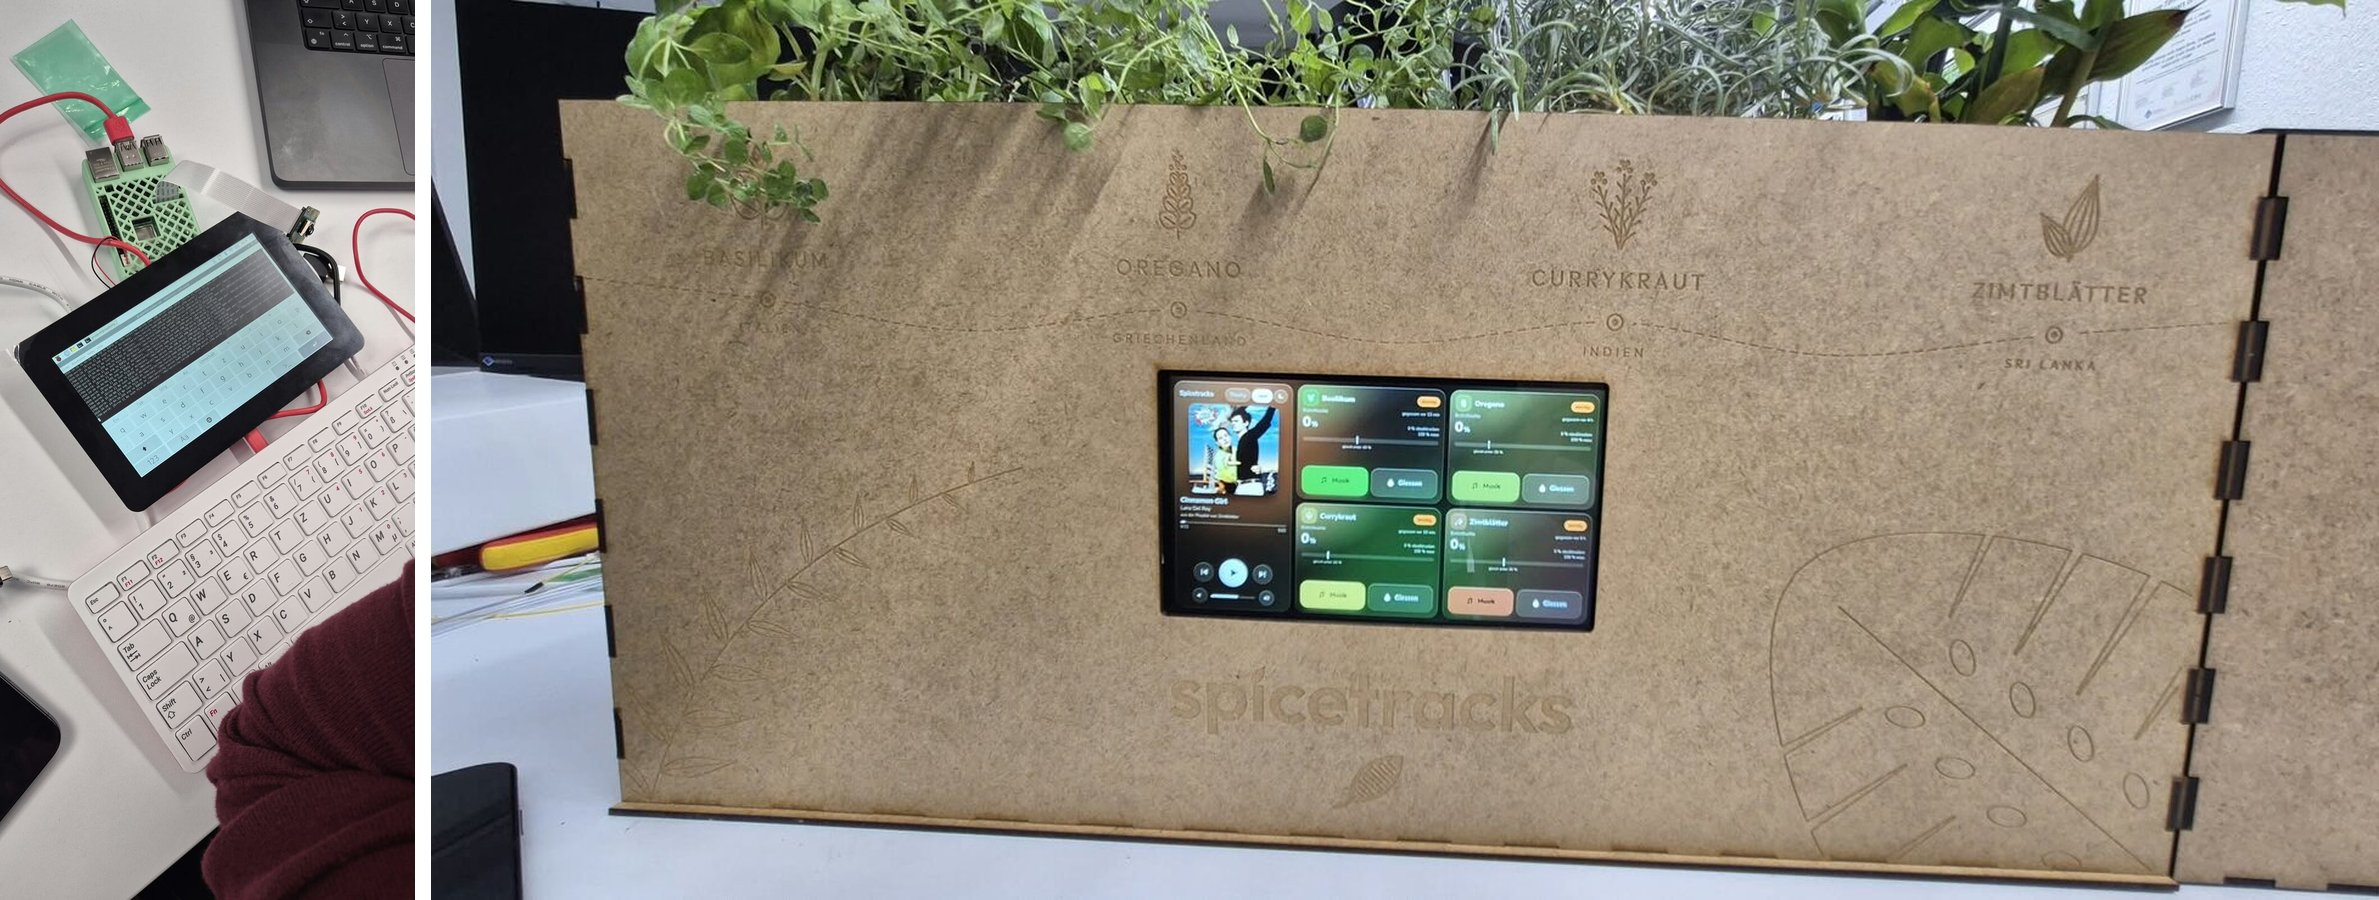
\includegraphics[width=\linewidth]{musik.jpg}
\caption{Erster Test des Displays am Raspberry Pi (links) und die Oberfläche im fertigen Gehäuse (rechts).}
\label{fig:display}
\end{figure}

\subsection{Software}

Wie die Hardware ist auch der Code auf zwei Programme verteilt. Die Firmware für den ESP32 (aktuell Version 2.14) ist in Arduino/C++ geschrieben und nutzt Adafruit NeoPixel für die LEDs und ArduinoJson für die Nachrichten an den Pi. Das Programm auf dem Pi ist in Python geschrieben und startet als systemd-Dienst automatisch mit. Auf dem Display öffnet sich beim Start Chromium im Kiosk-Modus, sodass gleich die Oberfläche zu sehen ist. Die wichtigsten Dateien stehen in der Tabelle.

\begin{table}[H]
\centering
\small
\begin{tabularx}{\linewidth}{>{\raggedright\arraybackslash\footnotesize}p{9.7cm}L}
\toprule
\textbf{Datei im Repository} & \textbf{Inhalt} \\
\midrule
\path{software/firmware/spicetracks_esp32/spicetracks_esp32.ino} & Firmware ESP32: Sensoren, Pumpe, Motor, LEDs, Protokoll \\
\path{software/firmware/spicetracks_esp32/touch_lukas.h} & Touch-Erkennung Version 4 \\
\path{software/pi/config.yaml} & Pflanzen, Farben, Grenzwerte, Playlists, Touch-Empfindlichkeit, Equalizer an oder aus, Demo-Modus für Vorführungen \\
\path{software/pi/spicetracks/app.py} & Logik: Touch, Musik, Giessen, Licht \\
\path{software/pi/spicetracks/esp_link.py} & serielle Verbindung zum ESP32 \\
\path{software/pi/spicetracks/spotify_ctl.py} & Spotify Web API \\
\path{software/pi/spicetracks/audio_eq.py} & Equalizer (FFT, Beat-Erkennung) \\
\path{software/pi/spicetracks/web.py} & Webserver für die Oberfläche \\
\path{software/pi/spicetracks/hwtest.py} & Testmenü für die Hardware \\
\path{software/pi/web/index.html} & Oberfläche auf dem Display \\
\bottomrule
\end{tabularx}
\end{table}

Alle Einstellungen stehen in einer einzigen Datei, der \path{config.yaml}: die Pflanzen mit Farben und Grenzwerten, die Helligkeit der LEDs, die Empfindlichkeit der Touch-Erkennung sowie die Schalter für den Equalizer und den Demo-Modus. Das Programm liest die Datei alle 10\,s neu ein. Farben oder Grenzwerte kann man also ändern, ohne etwas neu zu starten.

Beim Entwickeln half ausserdem, dass sich die Software auch ohne Hardware testen lässt. Dann ersetzt ein simulierter ESP32 die echte Elektronik, und die Pflanzen werden über Knöpfe im Browser „berührt“. Für die echte Hardware gibt es ein eigenes Testmenü, mit dem man Sensoren, LEDs, Pumpe und Verteiler einzeln prüfen kann.

% ---------------------------------------------------------------
\section{Reflexion}

\subsection{Schwierigkeiten und Lösungen}

Probleme gab es einige. Die meisten lagen im Zusammenspiel der Module oder kamen von aussen, etwa von Spotify, und nur wenige an einem einzelnen Bauteil. In der Tabelle stehen die wichtigsten, mit Ursache und der Lösung, die am Ende funktioniert hat.

{\small
\begin{xltabular}{\linewidth}{>{\raggedright\arraybackslash}p{3.3cm}>{\raggedright\arraybackslash}p{5.4cm}L}
\toprule
\textbf{Problem} & \textbf{Ursache} & \textbf{Lösung} \\
\midrule
\endfirsthead
\toprule
\textbf{Problem} & \textbf{Ursache} & \textbf{Lösung} \\
\midrule
\endhead
\bottomrule
\endlastfoot
Touch löst ohne Berührung aus & Die Schrauben nehmen auch das 50-Hz-Brummen aus dem Stromnetz auf, und das sieht für den ESP32 wie eine Berührung aus. & Version 4 der Touch-Erkennung misst 100-mal im Abstand von 1\,ms und mittelt über diese 100\,ms, also genau fünf Netzperioden. Beim Start kalibriert sie sich 30\,s lang, die Schwelle richtet sich nach dem gemessenen Rauschen. \\
\addlinespace
Touch-Messung bricht ab & Ein eingeschalteter Feuchtesensor im selben Topf stört die Messung so stark, dass sie abbricht. Der Chip hält dann alle Kanäle an. & Die Feuchtesensoren sind nur noch alle 10\,min für etwa 2\,s an, Touch pausiert in dieser Zeit. Hängt ein Kanal trotzdem, erkennt die Firmware das, und die übrigen Pflanzen laufen weiter. \\
\addlinespace
Eine Hand löst mehrere Pflanzen aus & Wer eine Pflanze anfasst, verändert auch den Messwert der Nachbartöpfe. & Seit Firmware 2.12 zählt nur die Pflanze mit dem stärksten Ausschlag. Eine andere übernimmt erst, wenn ihr Signal 1,5-mal stärker ist. Die Empfindlichkeit lässt sich in der \path{config.yaml} einstellen. \\
\addlinespace
Wasser trifft nicht alle Töpfe & Der erste, gerade Verteiler (gelbes Teil) passte nicht zum Arm, der sich im Halbkreis bewegt. An den beiden Enden lief der Arm am Verteiler vorbei. & Ein neuer, gebogener Verteiler (schwarzes Teil) folgt genau dem Weg des Arms und hat pro Pflanze eine Vertiefung. \\
\addlinespace
Ast passt nicht in den Drucker & Der gewählte Ast ist länger als der Druckraum des 3D-Druckers. & Der Ast ist in drei Teile zerlegt, die nach dem Druck zusammengesteckt werden. Zusammen mit Stämmen und Füssen passt alles auf fünf Druckplatten. \\
\addlinespace
LEDs brauchen zu viel Strom & Bei voller Helligkeit brauchen 40 LEDs deutlich mehr Strom, als das Netzteil-Modul auf dem Breadboard liefert (etwa 700\,mA). & Die LEDs hängen an einer eigenen Powerbank, die höchstens 2,4\,A liefert. Die Firmware begrenzt ihren Strom auf 1,5\,A. \\
\addlinespace
LEDs bleiben nach dem Löten dunkel & Ein Jumperkabel war defekt. Gefunden haben wir es erst nach langem Messen mit dem Multimeter. & Das Kabel wurde durch ein neues ersetzt. \\
\addlinespace
LEDs leuchten nur Blau, Rot und Weiss statt bunt & Geliefert wurde ein RGBW- statt des bestellten RGB-Streifens, in einem unbeschrifteten Plastiksack. Er erwartet 4 statt 3 Byte pro LED, deshalb verschoben sich die Farben von LED zu LED. & Kein Hardwarefehler: Nach mehreren Stunden Suche wurde die Firmware auf RGBW umgestellt, seither stimmen die Farben. \\
\addlinespace
Relais, Motor und LEDs schalten mal richtig und mal nicht & Die Masse des ESP32 war nicht mit der Masse des zweiten Breadboards verbunden. & Ein zusätzliches Kabel verbindet die beiden, seither läuft alles stabil. \\
\addlinespace
Musik spielt nicht auf dem Pi & librespot sollte den Pi zum Spotify-Lautsprecher machen. Spotify gibt den nötigen Audio-Schlüssel für viele Konten aber nicht mehr heraus. & Die Musik läuft im Browser auf dem Display über das offizielle Web Playback SDK, mit Widevine für die geschützte Wiedergabe. Gesteuert wird sie über die Web API. \\
\addlinespace
Keine Taktdaten für den Equalizer & Die Audioanalyse von Spotify, die Takt und Lautstärke eines Songs liefern sollte, gibt es nicht mehr. & Der Pi hört über den PipeWire-Monitor selbst mit, berechnet die Frequenzbänder per FFT und erkennt die Bass-Schläge. So braucht der Equalizer keine Daten von Spotify. \\
\addlinespace
Beim Pflanzenwechsel läuft kurz der alte Song & Spotify braucht nach einem Befehl einen Moment. Ein früherer Zwischenschritt in der Software startete ausserdem kurz den alten Song neu. & Der Player auf dem Display stoppt den alten Song sofort, und das Licht wechselt schon, bevor Spotify antwortet. Den Zwischenschritt gibt es nicht mehr. \\
\addlinespace
Musik ruckelt & Unschärfe und bewegte Farbflächen auf der Oberfläche brauchen viel Grafikleistung des Pi~4. Vermutlich kommt die gemeinsame Funkverbindung von WLAN und Bluetooth dazu. & Auf dem Pi läuft eine schlichtere Oberfläche ohne diese Effekte. Ganz behoben ist das Stocken damit nicht. \\
\addlinespace
Licht hinkt der Musik hinterher & Bluetooth-Lautsprecher spielen den Ton 150 bis 250\,ms später ab, als der Pi ihn verarbeitet. & Das Licht wartet 180\,ms, bevor es reagiert. So passt der Equalizer zu dem, was man hört. \\
\end{xltabular}}

Manche Probleme zeigten sich erst, als alle Module zusammen liefen. Dass die Feuchtesensoren die Touch-Messung stören, fiel zum Beispiel erst am letzten Kurstag auf. Gelöst haben wir es noch am selben Tag. Bei der Demo am Donnerstag machten die Touch-Sensoren noch Probleme, bei der finalen Demo am Freitag lief dann alles wie geplant.

\subsection{Was gut lief}

Die Pflanzen interaktiv zu machen, also genau das, worum es im Projekt geht, war überraschend einfach. Wir hatten damit viel mehr Aufwand erwartet. Am Ende reichten eine Schraube in der Erde und ein Touch-Pin am ESP32, und die Pflanze reagierte auf Berührung. Mehr Arbeit machte danach, dass die Erkennung nicht auf Störungen wie das Netzbrummen hereinfällt.

Gelohnt hat sich auch das schrittweise Vorgehen. Weil wir jedes Modul zuerst allein getestet haben, wussten wir bei einem Fehler im Gesamtsystem, dass die Teile an sich funktionieren, und mussten nur noch beim Zusammenspiel suchen. Geholfen hat auch, dass wir bei Bedarf in anderen Bereichen eingesprungen sind. So blieb kein Modul lange an einer Person hängen.

Auch das Drucken half beim Ausprobieren. Beim Verteiler zeigte das gelbe Testteil schnell, was nicht passt, bevor das schwarze gedruckt wurde. Beim Gehäuse war es ähnlich: Weil zuerst Probestücke geschnitten wurden, halten die gesteckten Fingerzinken jetzt ohne Leim.

In der Software hat sich bewährt, dass sie auch ohne Hardware läuft. Mit dem simulierten ESP32 und dem Testmenü liessen sich Software und Elektronik getrennt prüfen. Und weil das Programm die \path{config.yaml} laufend neu einliest, waren Farben, Grenzwerte und die Touch-Empfindlichkeit schnell nachjustiert, ohne dass etwas neu starten musste.

\subsection{Erkenntnisse}

Unterschätzt haben wir dagegen den Zusammenbau, also alles ins Gehäuse zu bringen und dann zu prüfen, ob es zusammen noch funktioniert. Einzeln liefen die Module meistens schnell. Sobald sie zusammenkamen, gab es neue Probleme, die vorher auf dem Tisch nicht aufgetaucht waren, etwa die fehlende gemeinsame Masse, die Stromversorgung der LEDs oder die Störung zwischen Feuchtesensoren und Touch. Beim nächsten Projekt würden wir für diese Phase von Anfang an deutlich mehr Zeit einplanen.

\begin{figure}[H]
\centering
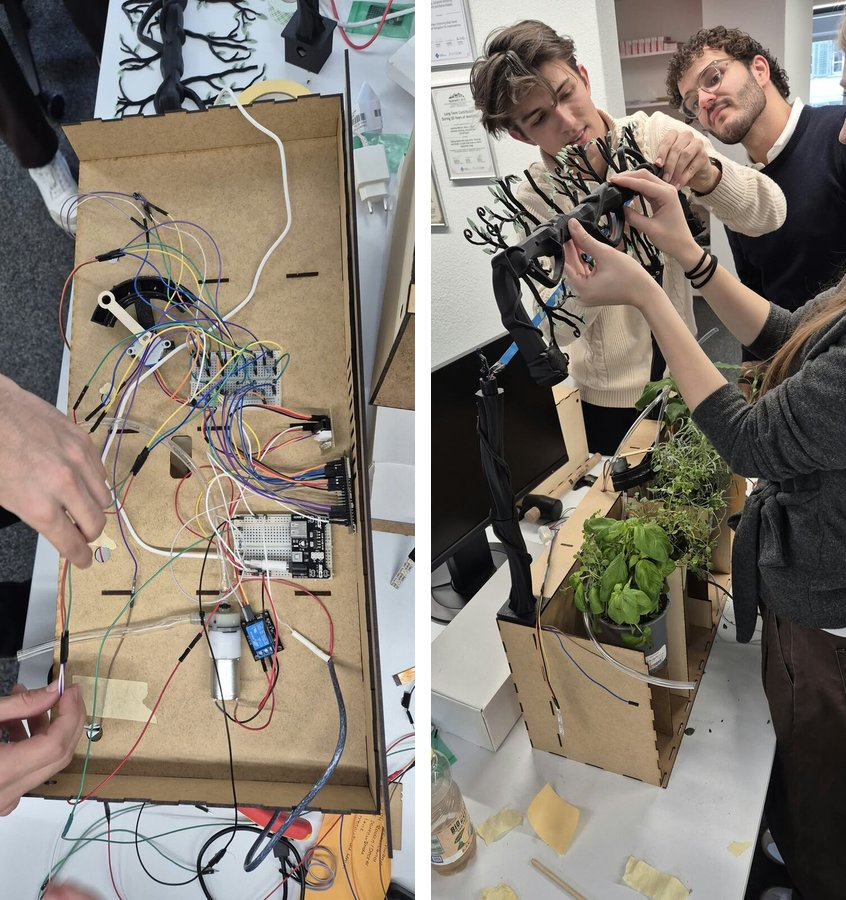
\includegraphics[width=0.55\linewidth]{zusammenbau.jpg}
\caption{Verkabelung im Inneren des Gehäuses (links) und Montage des Asts (rechts).}
\label{fig:zusammenbau}
\end{figure}

Daneben gibt es ein paar Dinge, die beim nächsten Projekt helfen würden. Lieferungen sollte man gleich beim Auspacken prüfen, gerade wenn sie nur in einem Plastiksack ohne Beschriftung kommen. Dass statt des bestellten RGB-Streifens ein RGBW-Streifen gekommen war, merkten wir erst nach Stunden an den falschen Farben. Und wenn etwas nicht funktioniert, liegt der Fehler nicht immer an der Hardware, nur weil man gerade gelötet hat. Bei den LEDs lag er am Ende in einer einzigen Einstellung in der Firmware.

Bei Diensten wie Spotify lohnt es sich, früh einen Plan B mitzudenken. Spotify hat das Projekt gleich an zwei Stellen eingeschränkt: librespot bekommt den nötigen Audio-Schlüssel nicht mehr, und die Audioanalyse steht neuen Apps nicht mehr zur Verfügung.

Sensoren sollte man früh zusammen testen und nicht nur jeden für sich. Die Feuchtesensoren haben die Touch-Messung gestört, und wer eine Pflanze berührt, lässt oft auch die Nachbartöpfe ausschlagen. Beides zeigte sich erst, als alles zusammen lief. Auch das Kalibrieren braucht Zeit, die man einplanen muss.

Die Stromversorgung gehört von Anfang an in die Planung, also wie viel Strom die LEDs brauchen und dass alle Teile eine gemeinsame Masse haben. Und die Bedienung muss man am echten Gerät ausprobieren. 

\subsection{Limitationen}

Bei der finalen Demo hat der Prototyp funktioniert, fertig ist er aber noch nicht. Einige Teile sind im Steckplan schon vorgesehen, aber noch nicht eingebaut. Es gibt zum Beispiel keinen Sensor für den Füllstand des Tanks, die Box merkt also nicht, wenn das Wasser ausgeht. Auch einen Endschalter hat der Verteiler nicht. Die Firmware zählt die Motorschritte ab der Stellung beim Einschalten, deshalb muss man den Arm vorher von Hand auf Pflanze 4 drehen.

Ausserdem reagiert die Box leicht verzögert, wenn man eine Pflanze berührt, und die Musik stockt manchmal. Ein Teil der Verzögerung kommt von Spotify selbst, das nach jedem Befehl einen Moment braucht. Für das Stocken gibt es zwei Verdächtige, die wir noch nicht genau gemessen haben: Der Pi~4 ist mit Display, Browser und Spotify-Player stark ausgelastet, und er schickt die Musik per Bluetooth an den Lautsprecher, während er sie gleichzeitig per WLAN lädt. Beim Pi~4 teilen sich WLAN und Bluetooth denselben Funkchip, was bekanntermassen zu Aussetzern führen kann. Ein Lautsprecher am Klinkenausgang wäre der einfachste nächste Test.

Eine Einschränkung kommt von Spotify. Wer die Spotify-App angelegt hat, braucht ein Premium-Konto, und seit März 2026 können solche Apps im Entwicklungsmodus höchstens fünf eingetragene Nutzer:innen haben. Für uns reicht das. Wollten mehr Leute die Box nutzen, wäre es ein Problem.

\subsection{Mögliche Erweiterungen}

Die naheliegenden Erweiterungen folgen direkt aus diesen Limitationen. Für einige sind im Steckplan schon Pins reserviert.

\begin{itemize}[itemsep=2pt]
  \item Füllstandssensor am Tank (GPIO 7 ist dafür vorgesehen), damit die Box vor einem leeren Tank warnt
  \item Endschalter am Verteiler (GPIO 39), damit der Arm seine Position nach jedem Start selbst findet
  \item Pegelwandler 74AHCT125 für das LED-Signal, falls die LEDs flackern
  \item Eine Kamera am Pi, mit der man die Pflanzen auch von woanders sieht und die einen zusätzlichen Hinweis auf ihren Zustand gibt. Sie war von Anfang an geplant (Abbildung~\ref{fig:skizzen}), wurde aber nicht umgesetzt.
\end{itemize}

% ---------------------------------------------------------------
\section{Anhang}

\subsection{Bestandteile des Portfolios}

\begin{table}[H]
\centering
\begin{tabularx}{\linewidth}{lL}
\toprule
\textbf{Teil} & \textbf{Ort im Repository} \\
\midrule
Videos & Nicht im Repository, da zu gross für GitHub. Produktvideo: \url{https://youtu.be/8oCQXXJ95Fs}, Behind the Scenes: \url{https://youtu.be/qCuY9ZzWwgk} \\
Code & \path{software/}: Firmware und Pi-Programm, mit README zum Einrichten und Testen; \path{tests/}: Testsketch für den ESP32 \\
Steckplan & \path{hardware/steckplan/}: \path{Group4-Spicetracks-Circuit-Diagram.html} und \path{.pdf}, mit Kabelliste \\
Lasercutter-Dateien & \path{hardware/laser/}: SVG-Dateien und Laserplan als PDF \\
3D-Druck-Dateien & \path{hardware/3d-druck/}: STL und 3MF, Druckplan als PDF \\
Prozessdokumentation & \path{docs/}: Fotos, Skizzen und die Abbildungen aus diesem Bericht \\
\bottomrule
\end{tabularx}
\end{table}

Alle Dateien sind im GitHub-Repository \url{https://github.com/KarlaRuggaber/hands-on-HCI} abgelegt.

\subsection{Nachbau in Kürze}

\begin{enumerate}[itemsep=2pt]
  \item Gehäuse aus den SVG-Dateien lasern und zusammenstecken, Ast in drei Teilen drucken.
  \item Elektronik nach dem Steckplan stecken, nur ohne Strom. Die roten Schienen der beiden Breadboards nie verbinden, gemeinsame Masse nicht vergessen.
  \item Firmware mit der Arduino IDE auf den ESP32-S3 laden (Board „ESP32S3 Dev Module“, Bibliotheken Adafruit NeoPixel und ArduinoJson 7).
  \item Auf dem Pi das Python-Programm installieren, eine Spotify-App anlegen, Playlists und Grenzwerte in \path{config.yaml} eintragen.
  \item Feuchtesensoren kalibrieren (Wert in der Luft und im Wasserglas ablesen) und die Teile einzeln mit dem Testmenü prüfen.
\end{enumerate}

Die genauen Schritte stehen im README unter \path{software/README.md}.

\subsection{Quellen}

Grundlage für das Projekt waren die Kursfolien von Hands-on HCI (Universität St.\,Gallen, Herbstsemester 2026, Katerina Koleva, Leon Reicherts und Gianluca Ielpo).

Während des ganzen Projekts haben wir den KI-Assistenten Claude (Anthropic) als Hilfsmittel eingesetzt, und zwar für viele verschiedene Aufgaben: beim Recherchieren von Dokumentationen und Datenblättern, bei der Fehlersuche an Hard- und Software, beim Schreiben und Überarbeiten von Code für die Firmware und das Programm auf dem Pi, beim Erstellen des interaktiven Steckplans und beim sprachlichen Überarbeiten dieses Berichts. Die Idee für Spicetracks, das Konzept und alle Gestaltungsentscheidungen stammen von uns. Wenn Claude technische Lösungswege vorgeschlagen hat, haben wir entschieden, welche wir umsetzen. Alle Ergebnisse haben wir selbst geprüft, am Prototyp getestet und wo nötig angepasst. Für den Prototyp und den Inhalt dieses Berichts tragen wir die Verantwortung.

Die wichtigsten Dokumentationen waren:

\begin{itemize}[itemsep=2pt]
  \item Raspberry Pi Documentation: \url{https://www.raspberrypi.com/documentation/computers/getting-started.html}
  \item Arduino Documentation: \url{https://docs.arduino.cc/}, für die Arduino IDE und die Programmierung des ESP32
  \item Dokumentation von Espressif zum ESP32-S3-DevKitC-1
  \item Bibliotheken Adafruit NeoPixel und ArduinoJson
  \item Spotify Web API und Spotify Web Playback SDK: \url{https://developer.spotify.com/documentation/web-api}
  \item Spotify for Developers, Änderungen an der Web API vom 27.~November 2024 (Audioanalyse): \url{https://developer.spotify.com/blog/2024-11-27-changes-to-the-web-api}
  \item Spotify for Developers, Update on Developer Access and Platform Security vom 6.~Februar 2026 (Premium-Pflicht, fünf Nutzer:innen): \url{https://developer.spotify.com/blog/2026-02-06-update-on-developer-access-and-platform-security}
\end{itemize}

\end{document}